\documentclass[9pt]{article}
\usepackage[english]{babel}
\usepackage{amsmath,amsthm}
\usepackage{amsfonts}
\usepackage{graphicx}
\usepackage[margin=0.2in]{geometry}
\newcommand{\setlinespacing}[1]{\setlength{\baselineskip}{#1 \defbaselineskip}}
\newcommand{\doublespacing}{\setlength{\baselineskip}{2.0 \defbaselineskip}}
\newcommand{\singlespacing}{\setlength{\baselineskip}{\defbaselineskip}}
\newcommand{\A}{{\cal A}}
\newcommand{\h}{{\cal H}}
\newcommand{\s}{{\cal S}}
\newcommand{\W}{{\cal W}}
\newcommand{\BH}{\mathbf B(\cal H)}
\newcommand{\KH}{\cal  K(\cal H)}
\newcommand{\Real}{\mathbb R}
\newcommand{\Complex}{\mathbb C}
\newcommand{\Field}{\mathbb F}
\newcommand{\RPlus}{[0,\infty)}
\newcommand{\norm}[1]{\left\Vert#1\right\Vert}
\newcommand{\essnorm}[1]{\norm{#1}_{\text{\rm\normalshape ess}}}
\newcommand{\abs}[1]{\left\vert#1\right\vert}
\newcommand{\set}[1]{\left\{#1\right\}}
\newcommand{\seq}[1]{\left<#1\right>}
\newcommand{\eps}{\varepsilon}
\newcommand{\To}{\longrightarrow}
\newcommand{\RE}{\operatorname{Re}}
\newcommand{\IM}{\operatorname{Im}}
\newcommand{\Poly}{{\cal{P}}(E)}
\newcommand{\EssD}{{\cal{D}}}
\newcommand{\field}[1]{\mathbb{#1}}
\newcommand{\C}{\field{C}}
\newcommand{\R}{\field{R}}
\newcommand{\script}[1]{\mathcal{#1}}
\newcommand{\fall}{\; \forall \;}
\newcommand{\exts}{\; \exists \;}
\newcommand{\mbf}[1]{\mathbf{#1}}
\newcommand{\binomial}[2]{\biggl( \begin{array}{c}  #1 \\ #2  \\ \end{array} \biggr) }
\newcommand{\fderiv}[2]{ \frac{d}{ d #1} \: #2}
\newcommand{\sderiv}[2]{ \frac{d^2}{ d^2 #1} \: #2}
\newcommand{\pfderiv}[2]{ \frac{\partial}{ \partial #1} \: #2}
\newcommand{\psderiv}[2]{ \frac{\partial^2}{ \partial^2 #1} \: #2}
\newcommand{\mat}[1]{\mathbf{#1}}
\DeclareSymbolFont{AMSb}{U}{msb}{m}{n}
\DeclareMathSymbol{\dblz}{\mathalpha}{AMSb}{"5A}
\DeclareMathSymbol{\dblr}{\mathalpha}{AMSb}{"52}
\DeclareMathSymbol{\dblt}{\mathalpha}{AMSb}{"54}
\DeclareMathSymbol{\dblq}{\mathalpha}{AMSb}{"51}
\DeclareMathSymbol{\dbln}{\mathalpha}{AMSb}{"4E}
\DeclareMathSymbol{\dblf}{\mathalpha}{AMSb}{"46}
\DeclareMathSymbol{\dblc}{\mathalpha}{AMSb}{"43}
\DeclareMathSymbol{\dbld}{\mathalpha}{AMSb}{"44}
\theoremstyle{plain}
\newtheorem{thm}{Theorem}[section]
\newtheorem{cor}[thm]{Corollary}
\newtheorem{lem}[thm]{Lemma}
\newtheorem{prop}[thm]{Proposition}
\theoremstyle{definition}
\newtheorem{defn}{Definition}[section]
\theoremstyle{remark}
\newtheorem{rem}{Remark}[section]
\numberwithin{equation}{section}
\renewcommand{\theequation}{\thesection.\arabic{equation}}
\begin{document}
\title{Regression of KL Software Distribution   }
\author{KL Software Libraries}
\date{Tue Apr 22 22:00:00 2014
}
\maketitle
\textbf{ KL Library test output.  This LaTex file and the associated diagrams are produced by the KL software libraries.}
\subsubsection{Gram Matrix Consistency Check}
Sample Size = 4096
Feature dim = 3

$$Sigma$ = \left(
\begin{array}{
ccc}
+1.140 & +1.535 & +0.581 \\
+1.535 & +9.988 & +1.605 \\
+0.581 & +1.605 & +0.428 \\
\end{array}
\right)$ \newline 

$Sample Covariance = \left(
\begin{array}{
ccc}
+1.139 & +1.522 & +0.578 \\
+1.522 & +9.722 & +1.575 \\
+0.578 & +1.575 & +0.424 \\
\end{array}
\right)$ \newline 

$Sample Mean = \left(
\begin{array}{
ccc}
+1.01386 & +0.99111 & +1.00460 \\
\end{array}
\right)$ \newline 

$Sample Covariance-$Omega$ = \left(
\begin{array}{
ccc}
-0.001 & -0.013 & -0.003 \\
-0.013 & -0.267 & -0.031 \\
-0.003 & -0.031 & -0.004 \\
\end{array}
\right)$ \newline 

$Sample Covariance Eigs = \left(
\begin{array}{
ccc}
(+10.26072,+0.00000) & (+0.98334,+0.00000) & (+0.04047,+0.00000) \\
\end{array}
\right)$ \newline 

$Centered Mean = \left(
\begin{array}{
ccc}
+0.00000 & +0.00000 & +0.00000 \\
\end{array}
\right)$ \newline 

$Centered Covariance = \left(
\begin{array}{
ccc}
+1.139 & +1.522 & +0.578 \\
+1.522 & +9.722 & +1.575 \\
+0.578 & +1.575 & +0.424 \\
\end{array}
\right)$ \newline 

$Gram Matrix Gf Not scaled by sample size = \left(
\begin{array}{
ccc}
+4665.379 & +6232.575 & +2367.225 \\
+6232.575 & +39820.325 & +6448.871 \\
+2367.225 & +6448.871 & +1735.706 \\
\end{array}
\right)$ \newline 

$Gram Matrix Gf  scaled by sample size = \left(
\begin{array}{
ccc}
+1.139 & +1.522 & +0.578 \\
+1.522 & +9.722 & +1.574 \\
+0.578 & +1.574 & +0.424 \\
\end{array}
\right)$ \newline 

$SampleCovariance - Scaled Gf = \left(
\begin{array}{
ccc}
+0.000 & +0.000 & +0.000 \\
+0.000 & +0.002 & +0.000 \\
+0.000 & +0.000 & +0.000 \\
\end{array}
\right)$ \newline 

$EigenDecomp of SampleCovariance = \left(
\begin{array}{
ccc}
-0.173 & -0.971 & -0.166 \\
+0.918 & -0.219 & +0.331 \\
-0.357 & -0.095 & +0.929 \\
\end{array}
\right)$ \newline 

$EigenDecomp of Gram Matrix = \left(
\begin{array}{
ccc}
-0.117 & -0.975 & -0.188 \\
-0.303 & +0.215 & -0.928 \\
+0.946 & -0.051 & -0.321 \\
\end{array}
\right)$ \newline 

QueryPerformanceCounter  =  +64.019
\subsubsection{Solver }
\subsubsection{Haar Distributed Random Orthogonal Matrix $A \in O(n)$}
 Testing Operator Norm
Number of Dimensions: 8

$A = \left(
\begin{array}{
cccccccc}
+0.450 & +0.200 & -0.489 & -0.392 & +0.200 & -0.220 & +0.216 & +0.480 \\
+0.267 & +0.436 & +0.434 & +0.218 & +0.142 & -0.347 & +0.537 & -0.271 \\
+0.447 & -0.285 & +0.297 & -0.415 & +0.473 & +0.072 & -0.321 & -0.356 \\
+0.254 & +0.436 & +0.187 & -0.318 & -0.673 & -0.051 & -0.387 & -0.058 \\
+0.396 & -0.165 & -0.576 & +0.358 & -0.213 & -0.112 & -0.032 & -0.544 \\
-0.116 & -0.567 & +0.140 & -0.236 & -0.296 & -0.692 & +0.148 & +0.034 \\
+0.509 & -0.386 & +0.284 & +0.235 & -0.301 & +0.410 & +0.261 & +0.360 \\
+0.179 & +0.037 & +0.129 & +0.535 & +0.199 & -0.404 & -0.567 & +0.373 \\
\end{array}
\right)$ \newline 

$Det(A) :   A \in O(n)$ = (-1.000,+0.000)

$L = \left(
\begin{array}{
cccccccc}
+1.000 & +0.000 & +0.000 & +0.000 & +0.000 & +0.000 & +0.000 & +0.000 \\
-0.227 & +1.000 & +0.000 & +0.000 & +0.000 & +0.000 & +0.000 & +0.000 \\
+0.777 & -0.205 & +1.000 & +0.000 & +0.000 & +0.000 & +0.000 & +0.000 \\
+0.884 & -0.827 & +0.756 & +1.000 & +0.000 & +0.000 & +0.000 & +0.000 \\
+0.500 & -0.960 & -0.320 & +0.662 & +1.000 & +0.000 & +0.000 & +0.000 \\
+0.524 & -0.975 & -0.642 & -0.007 & +0.086 & +1.000 & +0.000 & +0.000 \\
+0.878 & -0.082 & -0.085 & +0.730 & -0.539 & +0.145 & +1.000 & +0.000 \\
+0.352 & -0.264 & -0.110 & -0.491 & -0.296 & +0.865 & +0.955 & +1.000 \\
\end{array}
\right)$ \newline 

$U = \left(
\begin{array}{
cccccccc}
+0.509 & -0.386 & +0.284 & +0.235 & -0.301 & +0.410 & +0.261 & +0.360 \\
+0.000 & -0.654 & +0.204 & -0.182 & -0.364 & -0.599 & +0.208 & +0.116 \\
+0.000 & +0.000 & -0.755 & +0.138 & -0.054 & -0.553 & -0.192 & -0.800 \\
+0.000 & +0.000 & +0.000 & -0.855 & +0.205 & -0.659 & +0.302 & +0.862 \\
+0.000 & +0.000 & +0.000 & +0.000 & -1.026 & -0.572 & -0.580 & -0.954 \\
+0.000 & +0.000 & +0.000 & +0.000 & +0.000 & -1.457 & +0.532 & -0.772 \\
+0.000 & +0.000 & +0.000 & +0.000 & +0.000 & +0.000 & -1.160 & -1.762 \\
+0.000 & +0.000 & +0.000 & +0.000 & +0.000 & +0.000 & +0.000 & +2.681 \\
\end{array}
\right)$ \newline 

$L * U  = \left(
\begin{array}{
cccccccc}
+0.509 & -0.386 & +0.284 & +0.235 & -0.301 & +0.410 & +0.261 & +0.360 \\
-0.116 & -0.567 & +0.140 & -0.236 & -0.296 & -0.692 & +0.148 & +0.034 \\
+0.396 & -0.165 & -0.576 & +0.358 & -0.213 & -0.112 & -0.032 & -0.544 \\
+0.450 & +0.200 & -0.489 & -0.392 & +0.200 & -0.220 & +0.216 & +0.480 \\
+0.254 & +0.436 & +0.187 & -0.318 & -0.673 & -0.051 & -0.387 & -0.058 \\
+0.267 & +0.436 & +0.434 & +0.218 & +0.142 & -0.347 & +0.537 & -0.271 \\
+0.447 & -0.285 & +0.297 & -0.415 & +0.473 & +0.072 & -0.321 & -0.356 \\
+0.179 & +0.037 & +0.129 & +0.535 & +0.199 & -0.404 & -0.567 & +0.373 \\
\end{array}
\right)$ \newline 

$Det(L) :    = (+1.000,+0.000)     Det(U) :    = (+1.000,+0.000)     Det(LU) :    = (+1.000,+0.000)$

$||A||_{L_1}$  = +2.707

$||A||_{L_{\infty}}$ = +2.745

$||A^{-1}||_{L_1}$  = +2.745

$||A^{-1}||_{L_{\infty}}$ = +2.707

$||A||_{L_{\infty}} * ||A^{-1}||_{L_{\infty}} = +7.431$

$||A||_{L_1} * ||A^{-1}||_{L_1} = +7.431$

Frobenious Norm  $||A||_{\textit{F}}$ via $\sum\limits_{i,j =0}^{n} \|A_{i,j}|$   of  $A \in O(n)$  +2.828

$L_1$ condition number of Haar Distributed Random Orthogonal Matrix $A \in O(n)$ +6.033

$A = \left(
\begin{array}{
cccccccc}
+0.450 & +0.200 & -0.489 & -0.392 & +0.200 & -0.220 & +0.216 & +0.480 \\
+0.267 & +0.436 & +0.434 & +0.218 & +0.142 & -0.347 & +0.537 & -0.271 \\
+0.447 & -0.285 & +0.297 & -0.415 & +0.473 & +0.072 & -0.321 & -0.356 \\
+0.254 & +0.436 & +0.187 & -0.318 & -0.673 & -0.051 & -0.387 & -0.058 \\
+0.396 & -0.165 & -0.576 & +0.358 & -0.213 & -0.112 & -0.032 & -0.544 \\
-0.116 & -0.567 & +0.140 & -0.236 & -0.296 & -0.692 & +0.148 & +0.034 \\
+0.509 & -0.386 & +0.284 & +0.235 & -0.301 & +0.410 & +0.261 & +0.360 \\
+0.179 & +0.037 & +0.129 & +0.535 & +0.199 & -0.404 & -0.567 & +0.373 \\
\end{array}
\right)$ \newline 

$L_{\infty}$ condition number of Haar Distributed Random Orthogonal Matrix $A \in O(n)$ +6.798

Eigenvalues of $A \in O(n)$

(+0.616,+0.788), (+0.616,-0.788), (+0.261,+0.965), (+0.261,-0.965), (-0.580,+0.814), (-0.580,-0.814), (-1.000,+0.000), (+1.000,+0.000)

 $|\lambda | : \lambda \in \sigma(A) , A \in O(n)$

+1.000, +1.000, +1.000, +1.000, +1.000, +1.000, +1.000, +1.000


Calculating $A^{\dag} A,$  we expect $A^{\dag} A \approx I$

$A^{\dag} A = \left(
\begin{array}{
cccccccc}
+1.000 & +0.000 & -0.000 & -0.000 & +0.000 & -0.000 & +0.000 & +0.000 \\
+0.000 & +1.000 & -0.000 & -0.000 & -0.000 & -0.000 & -0.000 & +0.000 \\
-0.000 & -0.000 & +1.000 & +0.000 & -0.000 & +0.000 & +0.000 & -0.000 \\
-0.000 & -0.000 & +0.000 & +1.000 & +0.000 & -0.000 & -0.000 & -0.000 \\
+0.000 & -0.000 & -0.000 & +0.000 & +1.000 & -0.000 & +0.000 & -0.000 \\
-0.000 & -0.000 & +0.000 & -0.000 & -0.000 & +1.000 & +0.000 & -0.000 \\
+0.000 & -0.000 & +0.000 & -0.000 & +0.000 & +0.000 & +1.000 & +0.000 \\
+0.000 & +0.000 & -0.000 & -0.000 & -0.000 & -0.000 & +0.000 & +1.000 \\
\end{array}
\right)$ \newline 

Calculating $A^{-1} ,  A \in O(n)$.

$A^{-1} = \left(
\begin{array}{
cccccccc}
+0.450 & +0.267 & +0.447 & +0.254 & +0.396 & -0.116 & +0.509 & +0.179 \\
+0.200 & +0.436 & -0.285 & +0.436 & -0.165 & -0.567 & -0.386 & +0.037 \\
-0.489 & +0.434 & +0.297 & +0.187 & -0.576 & +0.140 & +0.284 & +0.129 \\
-0.392 & +0.218 & -0.415 & -0.318 & +0.358 & -0.236 & +0.235 & +0.535 \\
+0.200 & +0.142 & +0.473 & -0.673 & -0.213 & -0.296 & -0.301 & +0.199 \\
-0.220 & -0.347 & +0.072 & -0.051 & -0.112 & -0.692 & +0.410 & -0.404 \\
+0.216 & +0.537 & -0.321 & -0.387 & -0.032 & +0.148 & +0.261 & -0.567 \\
+0.480 & -0.271 & -0.356 & -0.058 & -0.544 & +0.034 & +0.360 & +0.373 \\
\end{array}
\right)$ \newline 

Calculating $A^{-1} *A  ,  A \in O(n)$.   We expect $A^{-1} *A  \approx I$. 

$A^{-1} *A = \left(
\begin{array}{
cccccccc}
+1.000 & +0.000 & -0.000 & -0.000 & +0.000 & -0.000 & +0.000 & -0.000 \\
+0.000 & +1.000 & +0.000 & +0.000 & +0.000 & -0.000 & +0.000 & -0.000 \\
+0.000 & +0.000 & +1.000 & -0.000 & +0.000 & -0.000 & +0.000 & -0.000 \\
+0.000 & -0.000 & -0.000 & +1.000 & -0.000 & -0.000 & -0.000 & -0.000 \\
+0.000 & -0.000 & -0.000 & -0.000 & +1.000 & +0.000 & -0.000 & -0.000 \\
+0.000 & -0.000 & +0.000 & -0.000 & +0.000 & +1.000 & -0.000 & +0.000 \\
+0.000 & +0.000 & -0.000 & +0.000 & -0.000 & +0.000 & +1.000 & +0.000 \\
-0.000 & +0.000 & +0.000 & +0.000 & -0.000 & +0.000 & -0.000 & +1.000 \\
\end{array}
\right)$ \newline 

Calculating SVD of  $A \in O(n)$

$U = \left(
\begin{array}{
cccccccc}
-0.450 & -0.200 & +0.489 & +0.392 & -0.200 & +0.220 & -0.216 & -0.480 \\
-0.261 & -0.446 & +0.242 & +0.048 & +0.043 & -0.538 & -0.249 & +0.564 \\
-0.292 & +0.545 & +0.238 & +0.272 & -0.082 & +0.304 & +0.243 & +0.574 \\
-0.265 & +0.509 & +0.024 & -0.404 & -0.481 & -0.446 & -0.211 & -0.178 \\
+0.631 & +0.040 & +0.692 & -0.230 & -0.145 & +0.112 & -0.161 & +0.093 \\
+0.115 & -0.369 & -0.213 & +0.066 & -0.825 & +0.132 & +0.279 & +0.160 \\
-0.386 & -0.241 & +0.033 & -0.720 & +0.076 & +0.499 & -0.048 & +0.126 \\
+0.117 & +0.099 & -0.346 & +0.176 & -0.116 & +0.303 & -0.825 & +0.199 \\
\end{array}
\right)$ \newline 

$S = \left(
\begin{array}{
cccccccc}
+1.000 & +0.000 & +0.000 & +0.000 & +0.000 & +0.000 & +0.000 & +0.000 \\
+0.000 & +1.000 & +0.000 & +0.000 & +0.000 & +0.000 & +0.000 & +0.000 \\
+0.000 & +0.000 & +1.000 & +0.000 & +0.000 & +0.000 & +0.000 & +0.000 \\
+0.000 & +0.000 & +0.000 & +1.000 & +0.000 & +0.000 & +0.000 & +0.000 \\
+0.000 & +0.000 & +0.000 & +0.000 & +1.000 & +0.000 & +0.000 & +0.000 \\
+0.000 & +0.000 & +0.000 & +0.000 & +0.000 & +1.000 & +0.000 & +0.000 \\
+0.000 & +0.000 & +0.000 & +0.000 & +0.000 & +0.000 & +1.000 & +0.000 \\
+0.000 & +0.000 & +0.000 & +0.000 & +0.000 & +0.000 & +0.000 & +1.000 \\
\end{array}
\right)$ \newline 

$V = \left(
\begin{array}{
cccccccc}
-1.000 & -0.000 & +0.000 & -0.000 & -0.000 & +0.000 & -0.000 & -0.000 \\
-0.000 & -0.243 & +0.180 & +0.095 & +0.265 & -0.265 & -0.573 & -0.656 \\
-0.000 & -0.076 & -0.627 & -0.217 & +0.530 & -0.461 & +0.247 & +0.009 \\
+0.000 & -0.169 & +0.033 & +0.726 & +0.530 & +0.239 & -0.033 & +0.323 \\
+0.000 & -0.400 & -0.582 & -0.092 & -0.265 & +0.318 & -0.529 & +0.202 \\
+0.000 & +0.648 & -0.437 & +0.255 & +0.000 & +0.350 & -0.015 & -0.450 \\
+0.000 & +0.023 & +0.192 & -0.577 & +0.530 & +0.589 & -0.049 & -0.020 \\
+0.000 & +0.572 & +0.081 & -0.104 & +0.132 & -0.301 & -0.572 & +0.470 \\
\end{array}
\right)$ \newline 

$U S V = \left(
\begin{array}{
cccccccc}
+0.450 & -0.112 & -0.390 & +0.409 & +0.288 & -0.048 & +0.609 & -0.098 \\
+0.261 & +0.032 & -0.023 & -0.116 & -0.034 & -0.473 & -0.011 & +0.832 \\
+0.292 & +0.368 & -0.034 & +0.082 & +0.641 & -0.139 & -0.564 & -0.156 \\
+0.265 & -0.260 & +0.483 & -0.180 & -0.075 & -0.622 & +0.101 & -0.440 \\
-0.631 & +0.156 & -0.422 & -0.188 & +0.221 & -0.514 & +0.186 & -0.127 \\
-0.115 & +0.608 & +0.559 & -0.009 & +0.212 & +0.112 & +0.486 & +0.105 \\
+0.386 & +0.541 & -0.349 & -0.418 & -0.457 & +0.009 & +0.053 & -0.223 \\
-0.117 & +0.310 & +0.034 & +0.755 & -0.444 & -0.301 & -0.164 & -0.061 \\
\end{array}
\right)$ \newline 

Calculating first few eigenvectors of $A \in O(n)$ using LAPACK syevx

\subsubsection{Wishart Matrix $A \in W(n)$}
$L_1$ condition number of Wishart Matrix +1489.694
$L_infty$ condition number of Wishart Matrix +1489.694
\subsubsection{Gaussian Orthogonal Ensemble $A \in GOE(n)$}
$L_1$ condition number of GOE Matrix +66.900
$L_\infty$ condition number of GOE Matrix +66.900
\subsubsection{The Identity Matrix $I \in M(n)$}
$L_1$ condition number of $I$ = +1.000
$L_\infty$ condition number of $I$ = +1.000
QueryPerformanceCounter  =  +2.038
\subsubsection{Generate Tracey Widom Sample}
\subsubsection{Sample from $W_n m$ times and calculate empirical PDF of the first eig}
Here we generate histograms of $\lambda_1$ for GOE (Gaussian Orthogonal Ensemble), and W (Wishart) 		 distributed of random matrices
These should approximate the celebrated Tracy Widom distribution.
Dimension $n = 128$

Sample size $m = 32$

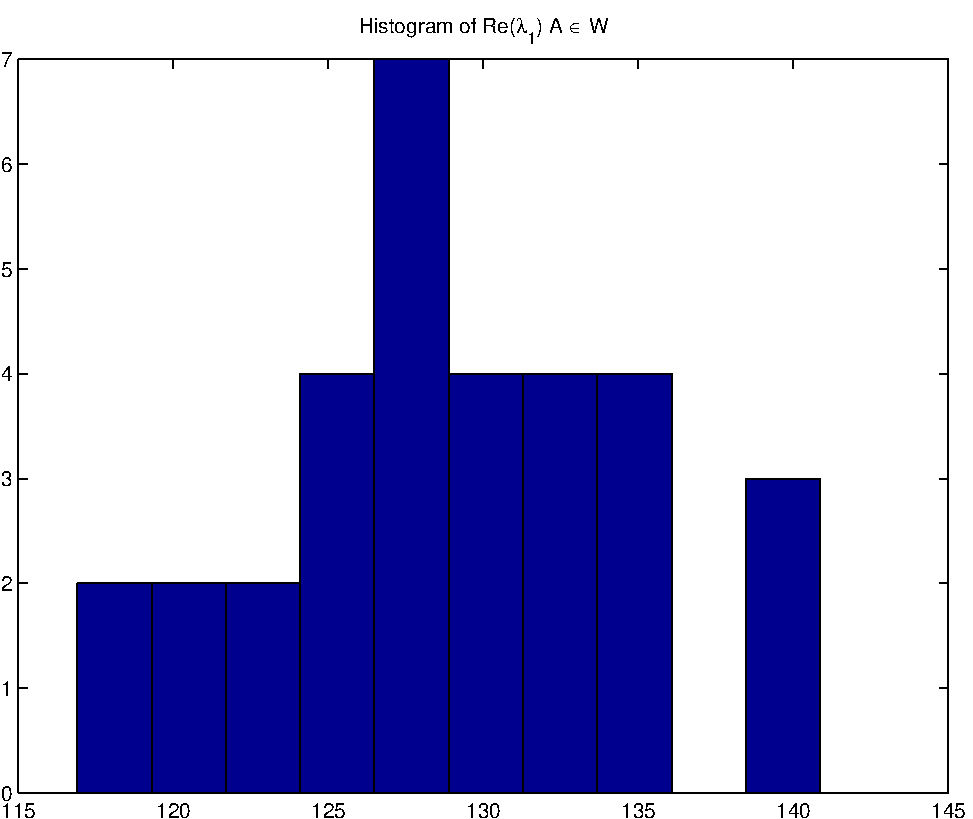
\includegraphics[width=10.0cm,height=10.0cm]{Re_TraceyWidom.pdf}

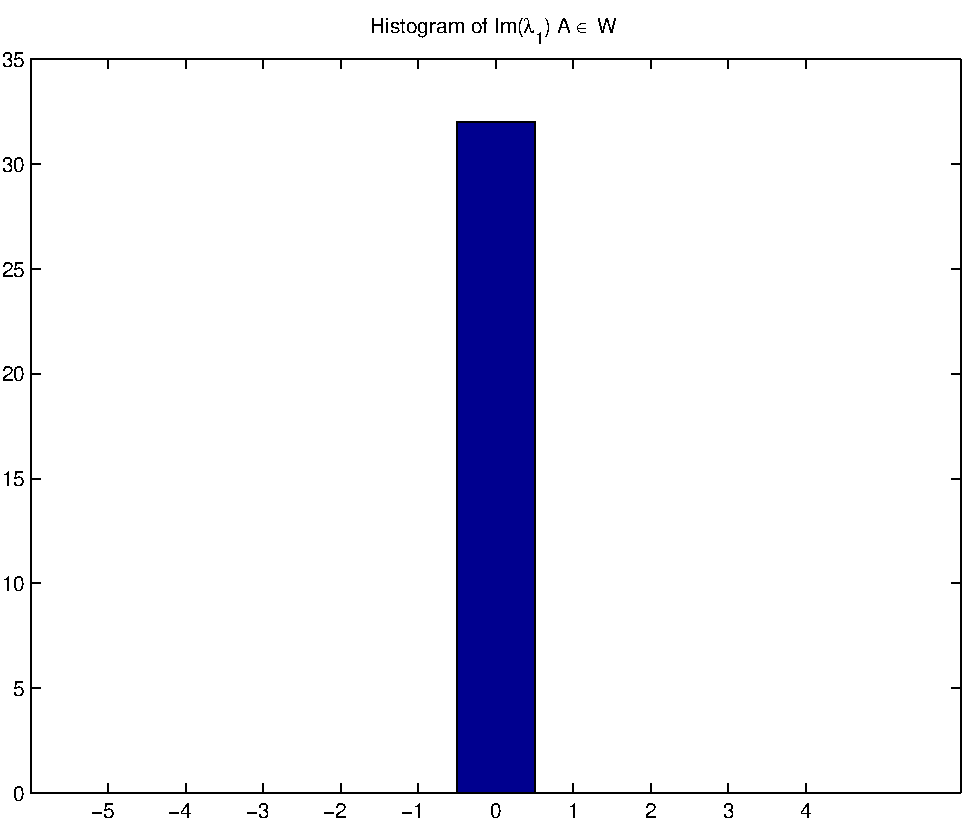
\includegraphics[width=10.0cm,height=10.0cm]{Im_TraceyWidom.pdf}

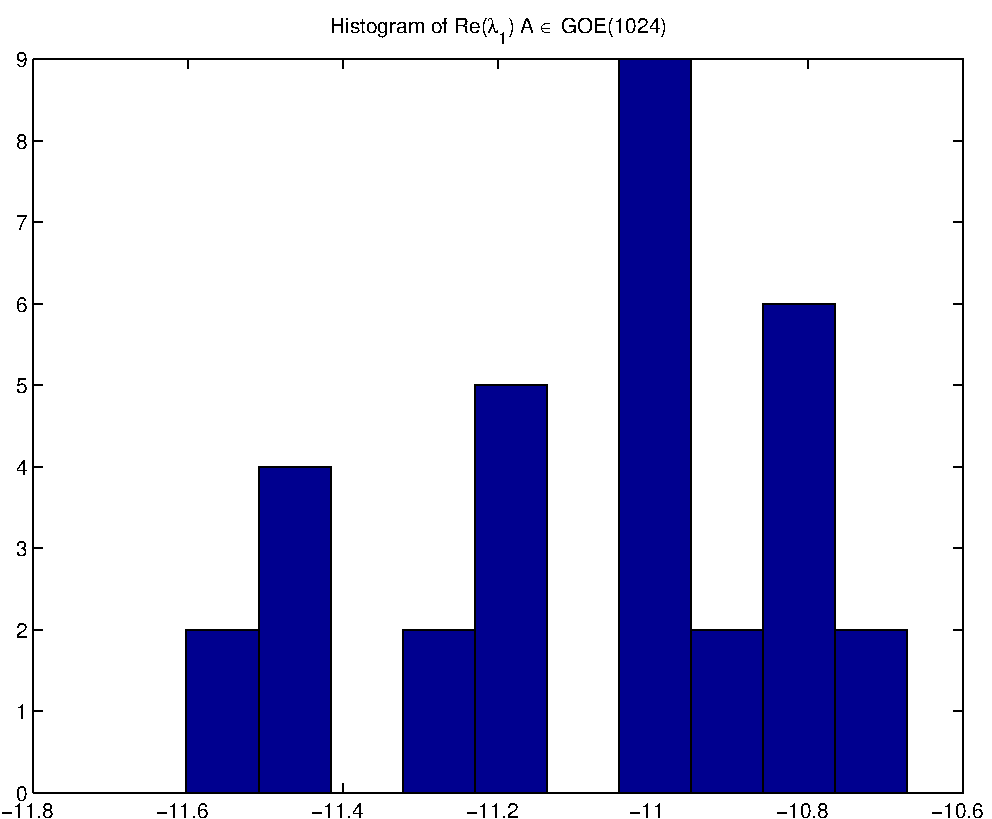
\includegraphics[width=10.0cm,height=10.0cm]{Re_Winger.pdf}

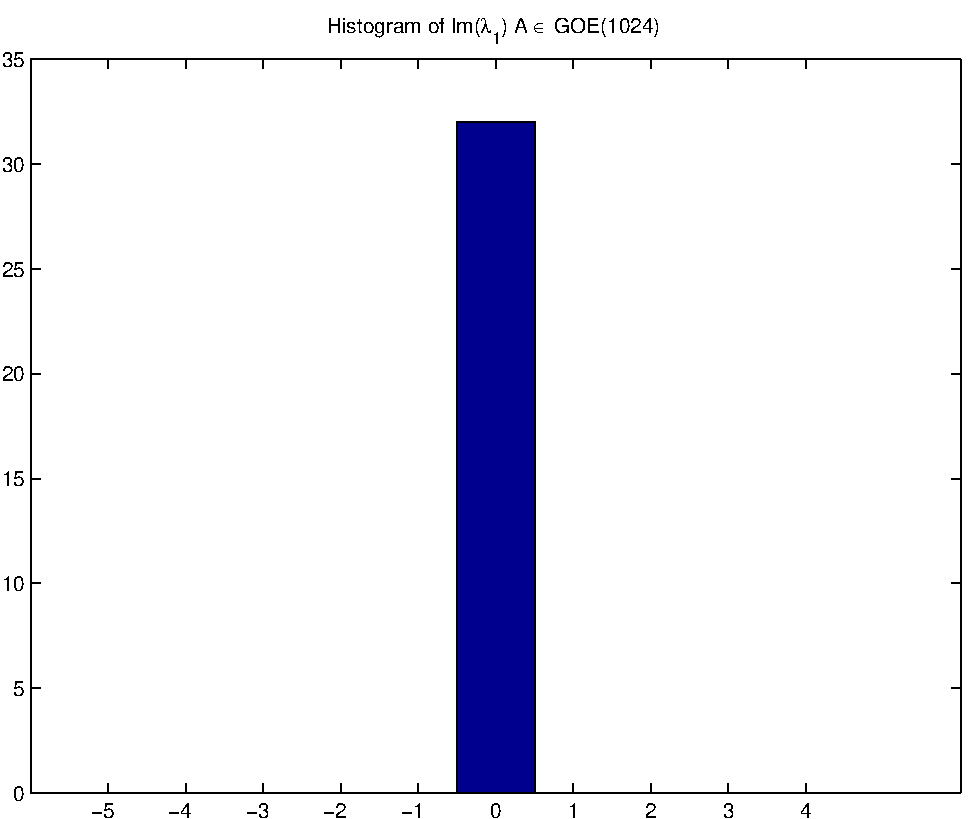
\includegraphics[width=10.0cm,height=10.0cm]{Im_Winger.pdf}

QueryPerformanceCounter  =  +12.031
\subsubsection{Approximate Winger Distribution}
\subsubsection{Verfy Winger Law.}
Let $M_n = [X_{ij} ]$ a symmetric n x n matrix with Random entries such that $X_{i,j} = X_{j,i}$, 		  and $X_{i,j}$ are iid $orall i < j,$ and $Xjj$ are iid $orall j  :  ; E[X^2_{ij} ] = 1, & E[X_{ij}] = 0$ 		  and that all moments exists for each of the entries.  		  The eigenvector of this random matrix; $ lambda_1 leq ... leq lambda_n$ depends continuously on $Mn$.
Dimension $n = 512$

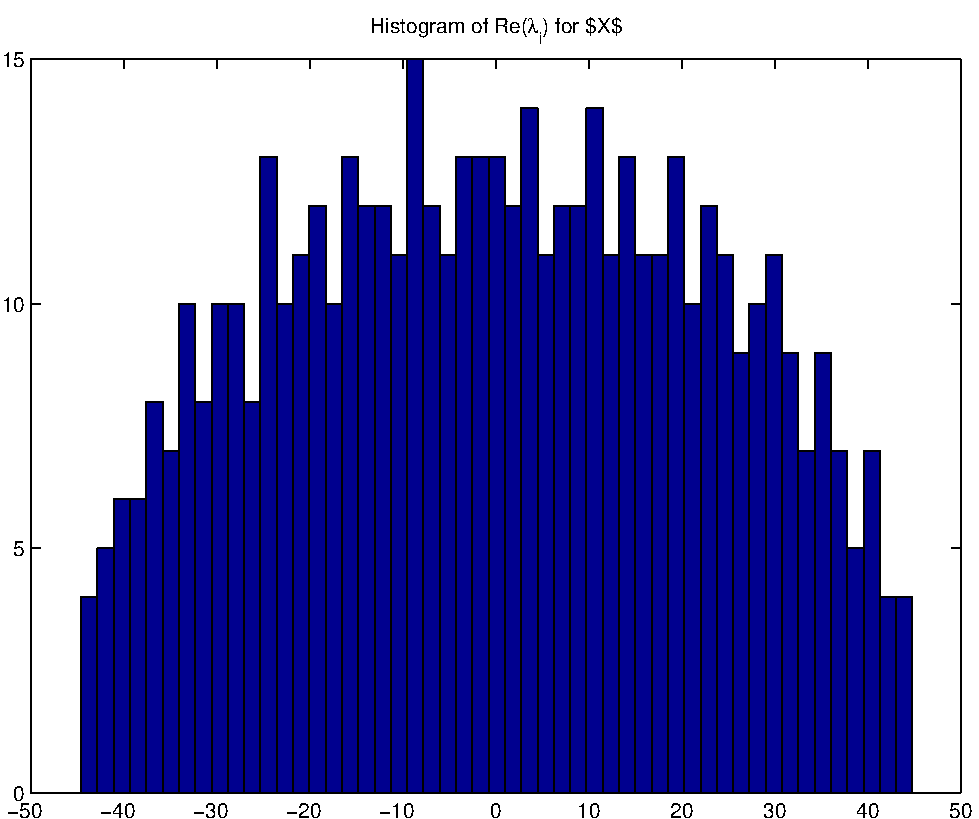
\includegraphics[width=10.0cm,height=10.0cm]{Re_lambda_n.pdf}

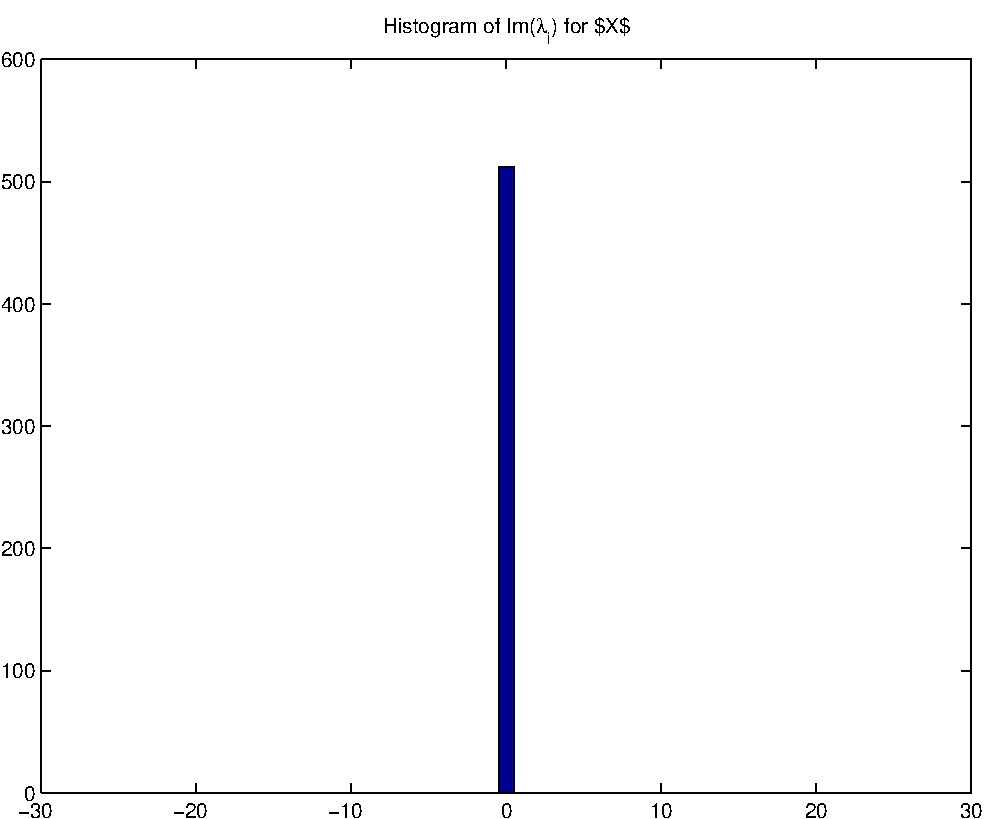
\includegraphics[width=10.0cm,height=10.0cm]{Im_lambda_n.pdf}

QueryPerformanceCounter  =  +2.693
\subsubsection{Iterated Exponential Filtering }
$\mu_1 =+0.093$
$\mu_2 =+0.726$
$\mu_3 =+0.011$
$\mu_4 =+2.178$
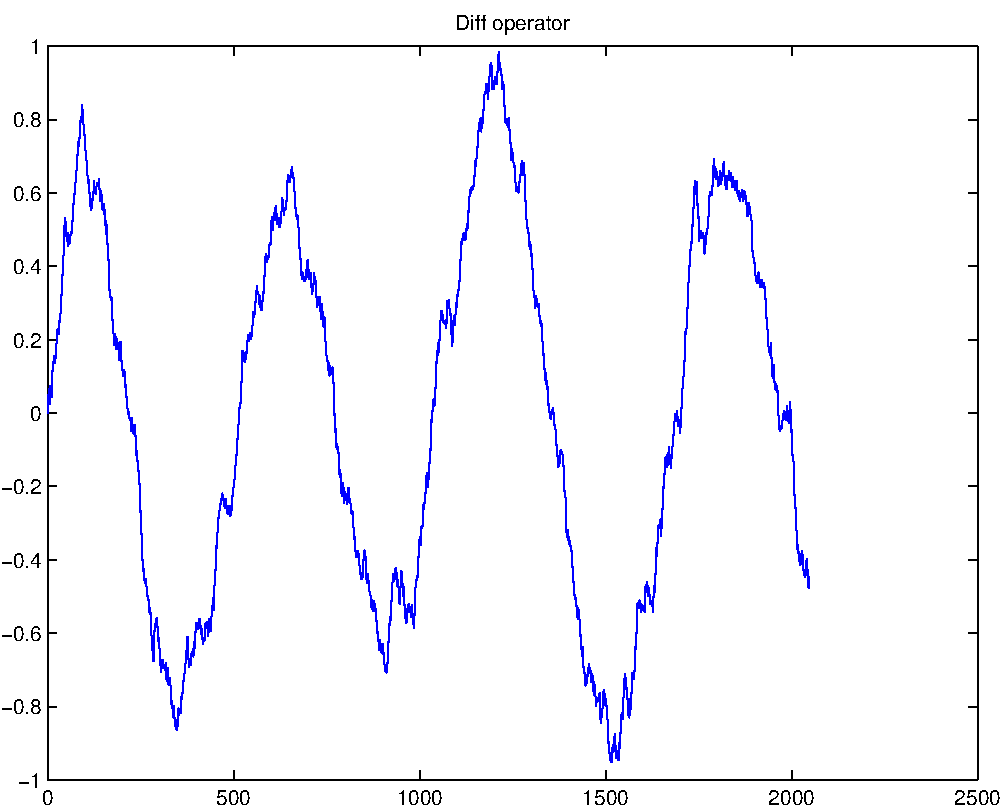
\includegraphics[width=10.0cm,height=10.0cm]{DIFF.pdf}

QueryPerformanceCounter  =  +1.601
\subsubsection{Matrix Exponential }
$SPD Matrix = \left(
\begin{array}{
cccccccc}
+10.539 & -0.499 & -0.010 & +0.368 & +0.465 & -0.492 & -0.126 & +0.437 \\
-0.499 & +7.286 & +0.365 & -0.481 & -0.337 & -0.466 & +0.279 & +0.056 \\
-0.010 & +0.365 & +6.705 & -0.205 & +0.467 & +0.131 & +0.077 & -0.089 \\
+0.368 & -0.481 & -0.205 & +6.496 & -0.402 & -0.209 & +0.043 & -0.041 \\
+0.465 & -0.337 & +0.467 & -0.402 & +4.578 & +0.272 & +0.289 & -0.285 \\
-0.492 & -0.466 & +0.131 & -0.209 & +0.272 & +8.181 & +0.343 & -0.244 \\
-0.126 & +0.279 & +0.077 & +0.043 & +0.289 & +0.343 & +5.938 & -0.212 \\
+0.437 & +0.056 & -0.089 & -0.041 & -0.285 & -0.244 & -0.212 & +9.691 \\
\end{array}
\right)$ \newline 

$SPD Eigs = \left(
\begin{array}{
cccccccc}
(+10.93611,+0.00000) & (+9.60778,+0.00000) & (+4.23666,+0.00000) & (+8.36911,+0.00000) & (+7.56229,+0.00000) & (+5.82791,+0.00000) & (+6.54198,+0.00000) & (+6.33139,+0.00000) \\
\end{array}
\right)$ \newline 

$exp(SPD) = \left(
\begin{array}{
cccccccc}
+47863.969 & -6460.093 & -1078.770 & +4706.958 & +2535.224 & -8475.398 & -2406.368 & +12977.552 \\
-6460.093 & +2780.574 & +516.920 & -1069.918 & -548.083 & -109.707 & +386.466 & -807.216 \\
-1078.770 & +516.920 & +1015.281 & -385.755 & +176.069 & +458.541 & +212.284 & -859.022 \\
+4706.958 & -1069.918 & -385.755 & +1267.210 & +111.181 & -1018.272 & -287.809 & +1036.628 \\
+2535.224 & -548.083 & +176.069 & +111.181 & +413.265 & +135.193 & +45.490 & -502.411 \\
-8475.398 & -109.707 & +458.541 & -1018.272 & +135.193 & +5613.026 & +968.003 & -4270.737 \\
-2406.368 & +386.466 & +212.284 & -287.809 & +45.490 & +968.003 & +632.432 & -1645.725 \\
+12977.552 & -807.216 & -859.022 & +1036.628 & -502.411 & -4270.737 & -1645.725 & +19362.944 \\
\end{array}
\right)$ \newline 

$exp(SPD) eigs = \left(
\begin{array}{
cccccccc}
(+56168.17045,+0.00000) & (+14880.07985,+0.00000) & (+4311.77579,+0.00000) & (+1924.25027,+0.00000) & (+69.17669,+0.00000) & (+339.64809,+0.00000) & (+693.66208,+0.00000) & (+561.93669,+0.00000) \\
\end{array}
\right)$ \newline 

$log(exp(SPD) eigs)  = \left(
\begin{array}{
cccccccc}
(+10.93611,+0.00000) & (+9.60778,+0.00000) & (+8.36911,+0.00000) & (+7.56229,+0.00000) & (+4.23666,+0.00000) & (+5.82791,+0.00000) & (+6.54198,+0.00000) & (+6.33139,+0.00000) \\
\end{array}
\right)$ \newline 

$exp(Id) = \left(
\begin{array}{
cccccccc}
+2.718 & +0.000 & +0.000 & +0.000 & +0.000 & +0.000 & +0.000 & +0.000 \\
+0.000 & +2.718 & +0.000 & +0.000 & +0.000 & +0.000 & +0.000 & +0.000 \\
+0.000 & +0.000 & +2.718 & +0.000 & +0.000 & +0.000 & +0.000 & +0.000 \\
+0.000 & +0.000 & +0.000 & +2.718 & +0.000 & +0.000 & +0.000 & +0.000 \\
+0.000 & +0.000 & +0.000 & +0.000 & +2.718 & +0.000 & +0.000 & +0.000 \\
+0.000 & +0.000 & +0.000 & +0.000 & +0.000 & +2.718 & +0.000 & +0.000 \\
+0.000 & +0.000 & +0.000 & +0.000 & +0.000 & +0.000 & +2.718 & +0.000 \\
+0.000 & +0.000 & +0.000 & +0.000 & +0.000 & +0.000 & +0.000 & +2.718 \\
\end{array}
\right)$ \newline 

$exp(Id) eigs = \left(
\begin{array}{
cccccccc}
(+2.71828,+0.00000) & (+2.71828,+0.00000) & (+2.71828,+0.00000) & (+2.71828,+0.00000) & (+2.71828,+0.00000) & (+2.71828,+0.00000) & (+2.71828,+0.00000) & (+2.71828,+0.00000) \\
\end{array}
\right)$ \newline 

$log(exp(Id) eigs)  = \left(
\begin{array}{
cccccccc}
(+1.00000,+0.00000) & (+1.00000,+0.00000) & (+1.00000,+0.00000) & (+1.00000,+0.00000) & (+1.00000,+0.00000) & (+1.00000,+0.00000) & (+1.00000,+0.00000) & (+1.00000,+0.00000) \\
\end{array}
\right)$ \newline 

For $n  \in  \dblz [16,128)$ we calculate  $|( SPD(n) Eigs - log(exp(SPD(n)) eigs)|_{l^2}$

$|( SPD(n) Eigs - log(exp(SPD(n)) eigs)|_{l^2} = \left(
\begin{array}{
cccccccccccccccccccccccccccccccccccccccccccccccccccccccccccccccccccccccccccccccccccccccccccccccccccccccccccccccc}
(+5.36543,+0.00000) & (+5.36543,+0.00000) & (+5.36543,+0.00000) & (+5.36543,+0.00000) & (+5.36543,+0.00000) & (+5.36543,+0.00000) & (+5.36543,+0.00000) & (+5.36543,+0.00000) & (+5.36543,+0.00000) & (+5.36543,+0.00000) & (+5.36543,+0.00000) & (+5.36543,+0.00000) & (+5.36543,+0.00000) & (+5.36543,+0.00000) & (+5.36543,+0.00000) & (+5.36543,+0.00000) & (+5.36543,+0.00000) & (+5.36543,+0.00000) & (+5.36543,+0.00000) & (+5.36543,+0.00000) & (+5.36543,+0.00000) & (+5.36543,+0.00000) & (+5.36543,+0.00000) & (+5.36543,+0.00000) & (+5.36543,+0.00000) & (+5.36543,+0.00000) & (+5.36543,+0.00000) & (+5.36543,+0.00000) & (+5.36543,+0.00000) & (+5.36543,+0.00000) & (+5.36543,+0.00000) & (+5.36543,+0.00000) & (+5.36543,+0.00000) & (+5.36543,+0.00000) & (+5.36543,+0.00000) & (+5.36543,+0.00000) & (+5.36543,+0.00000) & (+5.36543,+0.00000) & (+5.36543,+0.00000) & (+5.36543,+0.00000) & (+5.36543,+0.00000) & (+5.36543,+0.00000) & (+5.36543,+0.00000) & (+5.36543,+0.00000) & (+5.36543,+0.00000) & (+5.36543,+0.00000) & (+5.36543,+0.00000) & (+5.36543,+0.00000) & (+0.00000,+0.00000) & (+0.00000,+0.00000) & (+0.00000,+0.00000) & (+0.00000,+0.00000) & (+0.00000,+0.00000) & (+0.00000,+0.00000) & (+0.00000,+0.00000) & (+0.00000,+0.00000) & (+0.00000,+0.00000) & (+0.00000,+0.00000) & (+0.00000,+0.00000) & (+0.00000,+0.00000) & (+0.00000,+0.00000) & (+0.00000,+0.00000) & (+0.00000,+0.00000) & (+0.00000,+0.00000) & (+0.00000,+0.00000) & (+0.00000,+0.00000) & (+0.00000,+0.00000) & (+0.00000,+0.00000) & (+0.00000,+0.00000) & (+0.00000,+0.00000) & (+0.00000,+0.00000) & (+0.00000,+0.00000) & (+0.00000,+0.00000) & (+0.00000,+0.00000) & (+0.00000,+0.00000) & (+0.00000,+0.00000) & (+0.00000,+0.00000) & (+0.00000,+0.00000) & (+0.00000,+0.00000) & (+0.00000,+0.00000) & (+0.00000,+0.00000) & (+0.00000,+0.00000) & (+0.00000,+0.00000) & (+0.00000,+0.00000) & (+0.00000,+0.00000) & (+0.00000,+0.00000) & (+0.00000,+0.00000) & (+0.00000,+0.00000) & (+0.00000,+0.00000) & (+0.00000,+0.00000) & (+0.00000,+0.00000) & (+0.00000,+0.00000) & (+0.00000,+0.00000) & (+0.00000,+0.00000) & (+0.00000,+0.00000) & (+0.00000,+0.00000) & (+0.00000,+0.00000) & (+0.00000,+0.00000) & (+0.00000,+0.00000) & (+0.00000,+0.00000) & (+0.00000,+0.00000) & (+0.00000,+0.00000) & (+0.00000,+0.00000) & (+0.00000,+0.00000) & (+0.00000,+0.00000) & (+0.00000,+0.00000) & (+0.00000,+0.00000) & (+0.00000,+0.00000) & (+0.00000,+0.00000) & (+0.00000,+0.00000) & (+0.00000,+0.00000) & (+0.00000,+0.00000) \\
\end{array}
\right)$ \newline 

QueryPerformanceCounter  =  +0.03535
\subsubsection{Random Number Generator }
The sample size generated for this run is 100000.

\newpage
uniform \begin{tabular}{|c|c|c|c|}  mean & variance & skewness & kurtosis \\  \hline
$\mu_1 = +0.50030$ & $\mu_2 = +0.08353$ & $\mu_3 = +0.00339$ & $\mu_4 =+1.80113$ \\
\end{tabular}

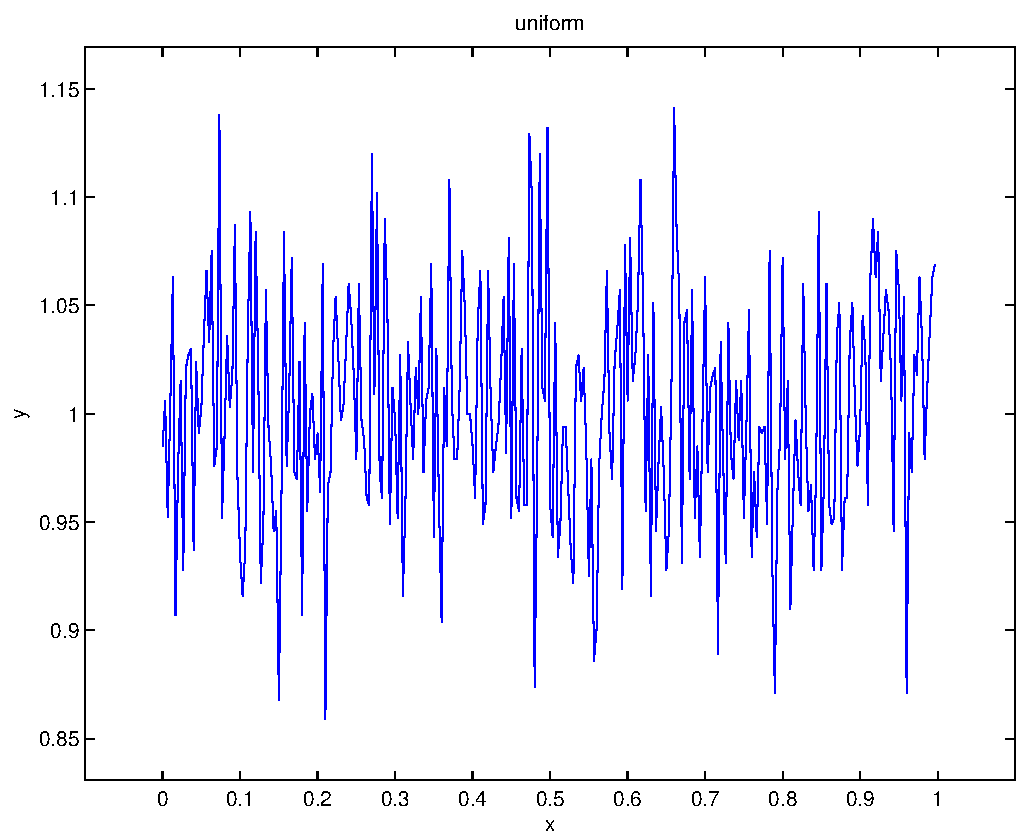
\includegraphics[width=5cm,height=5cm]{uniform.pdf}

cauchy \begin{tabular}{|c|c|c|c|}  mean & variance & skewness & kurtosis \\  \hline
$\mu_1 = +0.44288$ & $\mu_2 = +0.05341$ & $\mu_3 = +0.63935$ & $\mu_4 =+3.28094$ \\
\end{tabular}

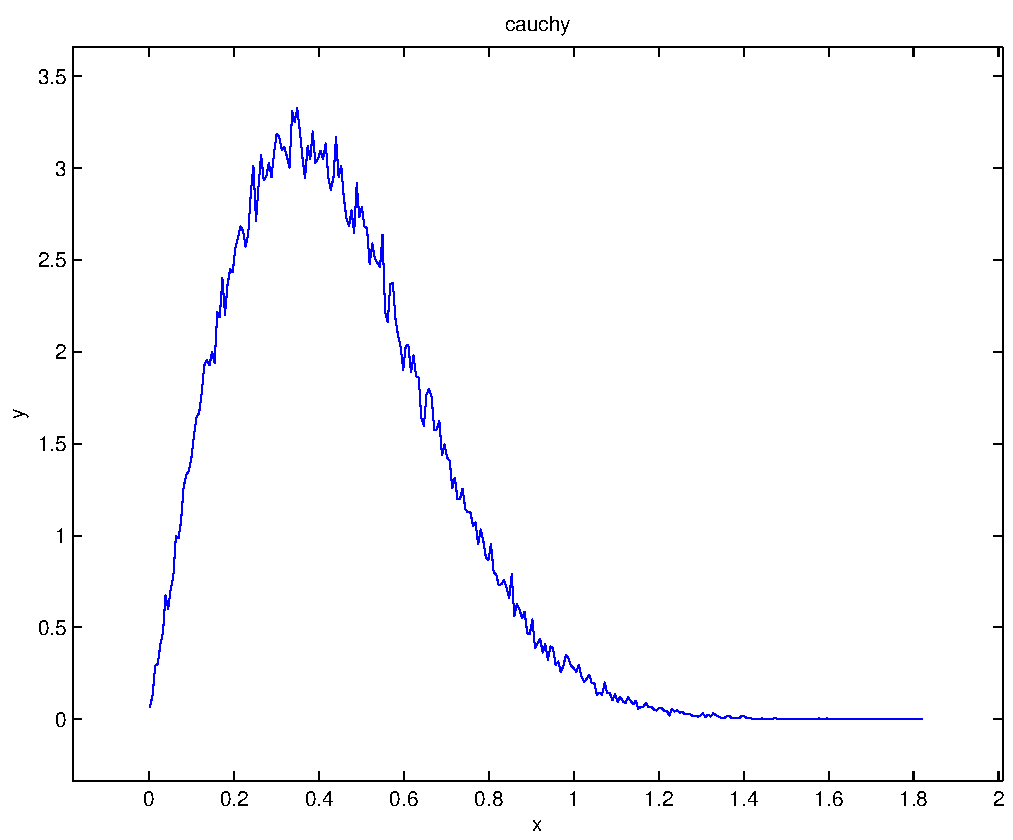
\includegraphics[width=5cm,height=5cm]{cauchy.pdf}

exponential \begin{tabular}{|c|c|c|c|}  mean & variance & skewness & kurtosis \\  \hline
$\mu_1 = +1.99647$ & $\mu_2 = +3.99339$ & $\mu_3 = +2.03097$ & $\mu_4 =+9.30842$ \\
\end{tabular}

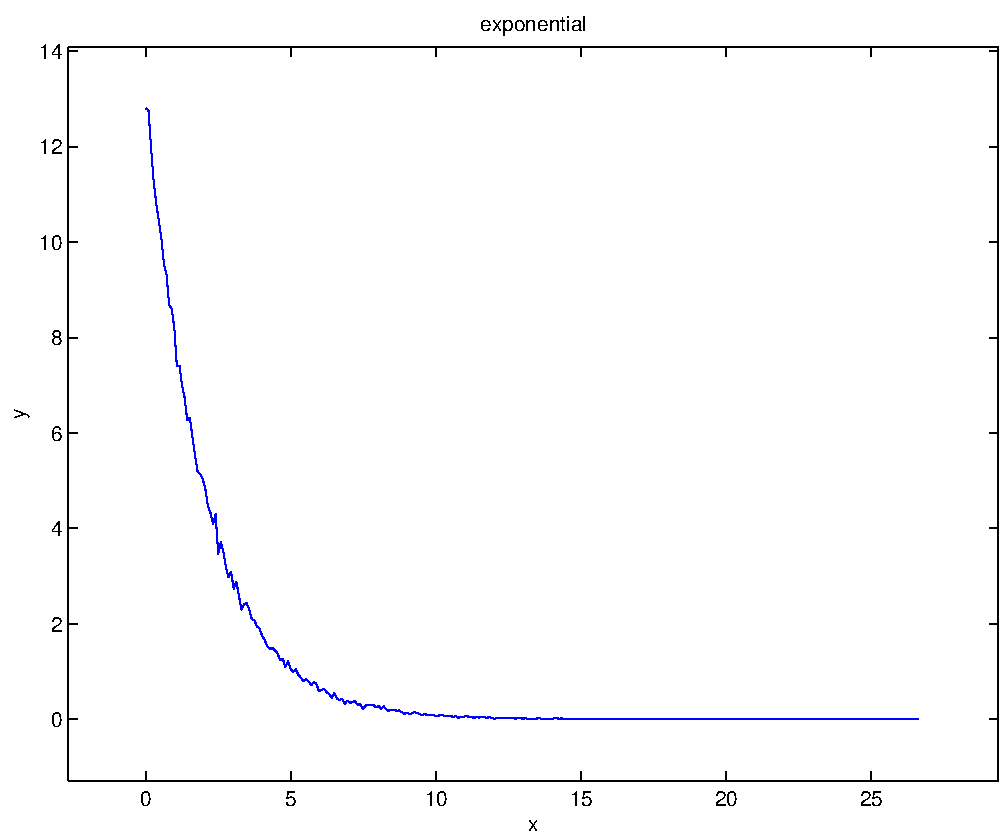
\includegraphics[width=5cm,height=5cm]{exponential.pdf}

\newpage
gamma \begin{tabular}{|c|c|c|c|}  mean & variance & skewness & kurtosis \\  \hline
$\mu_1 = +1.89052$ & $\mu_2 = +1.89855$ & $\mu_3 = +1.46712$ & $\mu_4 =+6.21783$ \\
\end{tabular}

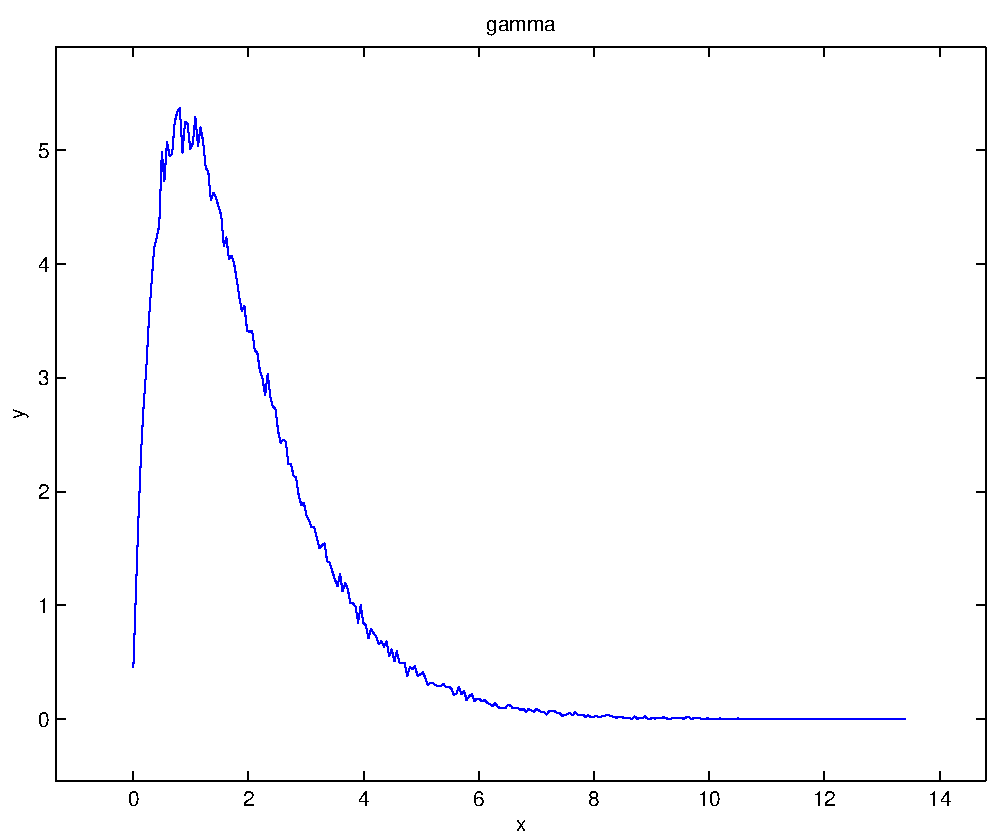
\includegraphics[width=5cm,height=5cm]{gamma.pdf}

GIG \begin{tabular}{|c|c|c|c|}  mean & variance & skewness & kurtosis \\  \hline
$\mu_1 = +0.80315$ & $\mu_2 = +11.22582$ & $\mu_3 = +15.31482$ & $\mu_4 =+317.47280$ \\
\end{tabular}

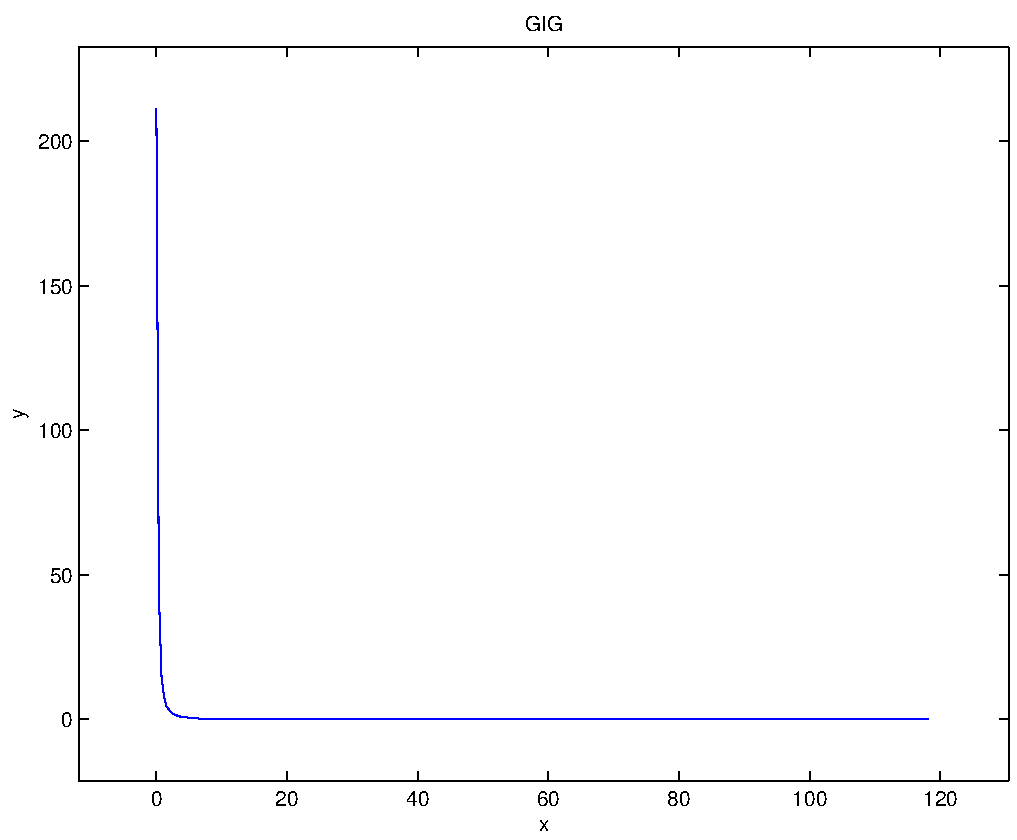
\includegraphics[width=5cm,height=5cm]{GIG.pdf}

normal-box-muller \begin{tabular}{|c|c|c|c|}  mean & variance & skewness & kurtosis \\  \hline
$\mu_1 = -0.00146$ & $\mu_2 = +0.99607$ & $\mu_3 = -0.00643$ & $\mu_4 =+2.98875$ \\
\end{tabular}

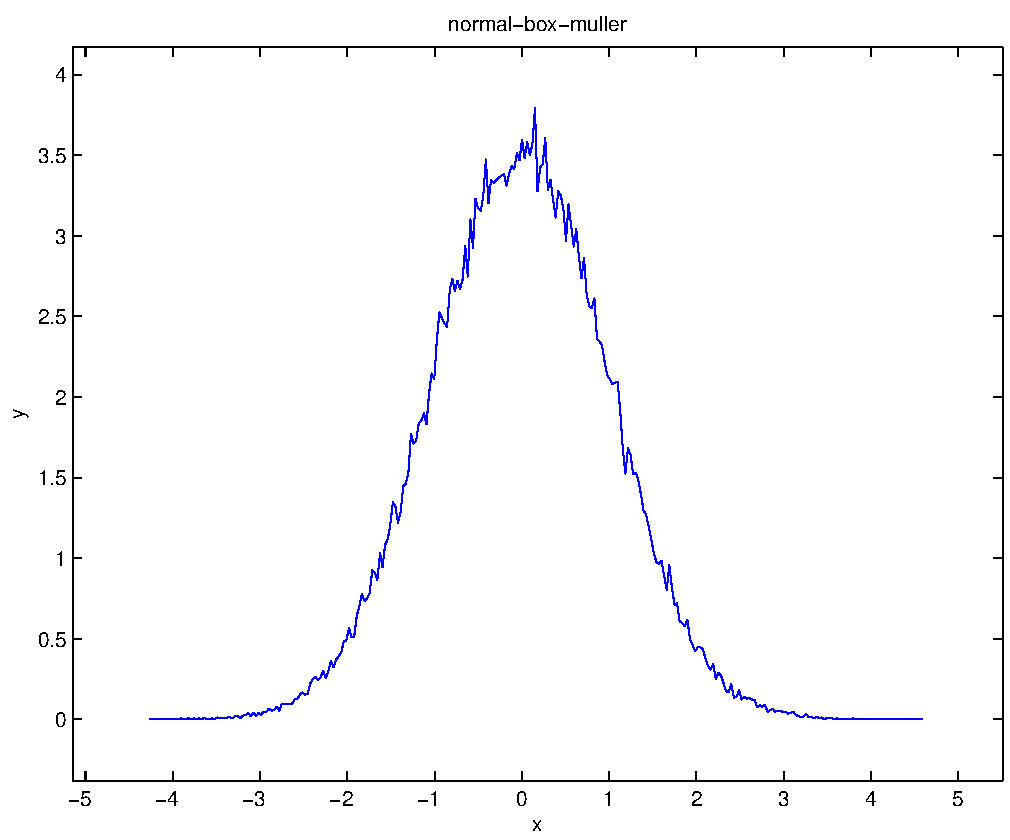
\includegraphics[width=5cm,height=5cm]{normal-box-muller.pdf}

\newpage
normal-inverse-approximation \begin{tabular}{|c|c|c|c|}  mean & variance & skewness & kurtosis \\  \hline
$\mu_1 = +0.00230$ & $\mu_2 = +1.00486$ & $\mu_3 = +0.01163$ & $\mu_4 =+2.99254$ \\
\end{tabular}

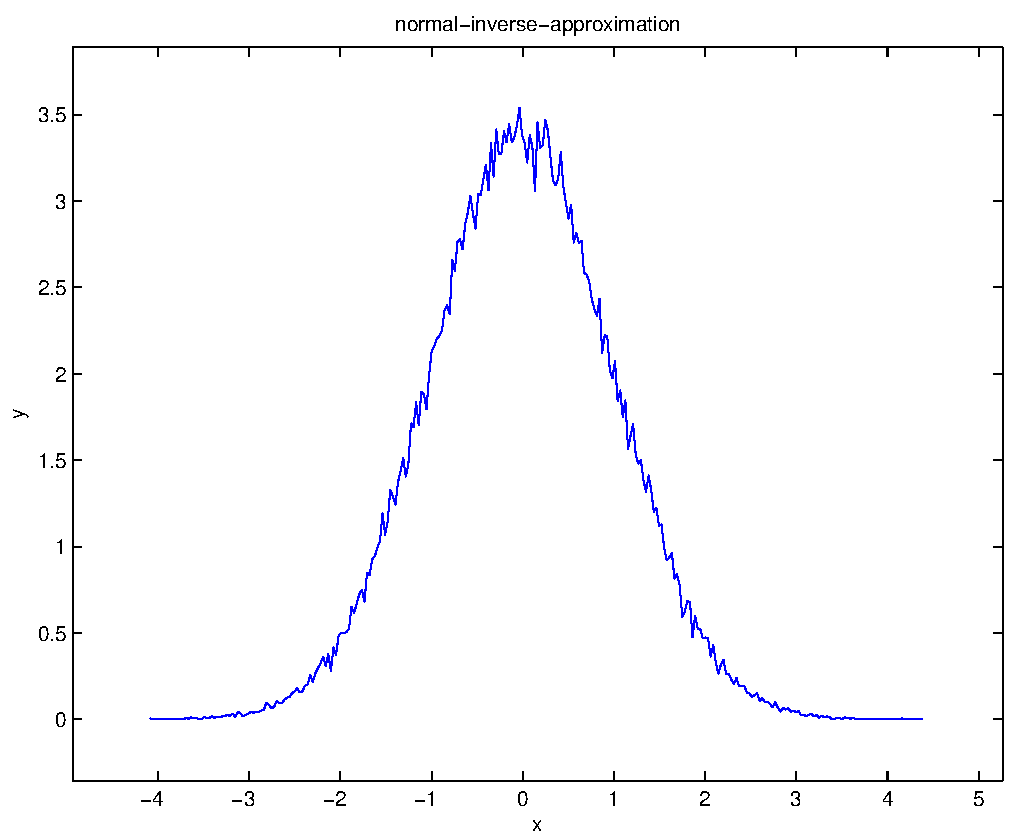
\includegraphics[width=5cm,height=5cm]{normal-inverse-approximation.pdf}

pareto \begin{tabular}{|c|c|c|c|}  mean & variance & skewness & kurtosis \\  \hline
$\mu_1 = +3184578.26493$ & $\mu_2 = +888468246174112900.00000$ & $\mu_3 = +315.36997$ & $\mu_4 =+99629.09819$ \\
\end{tabular}

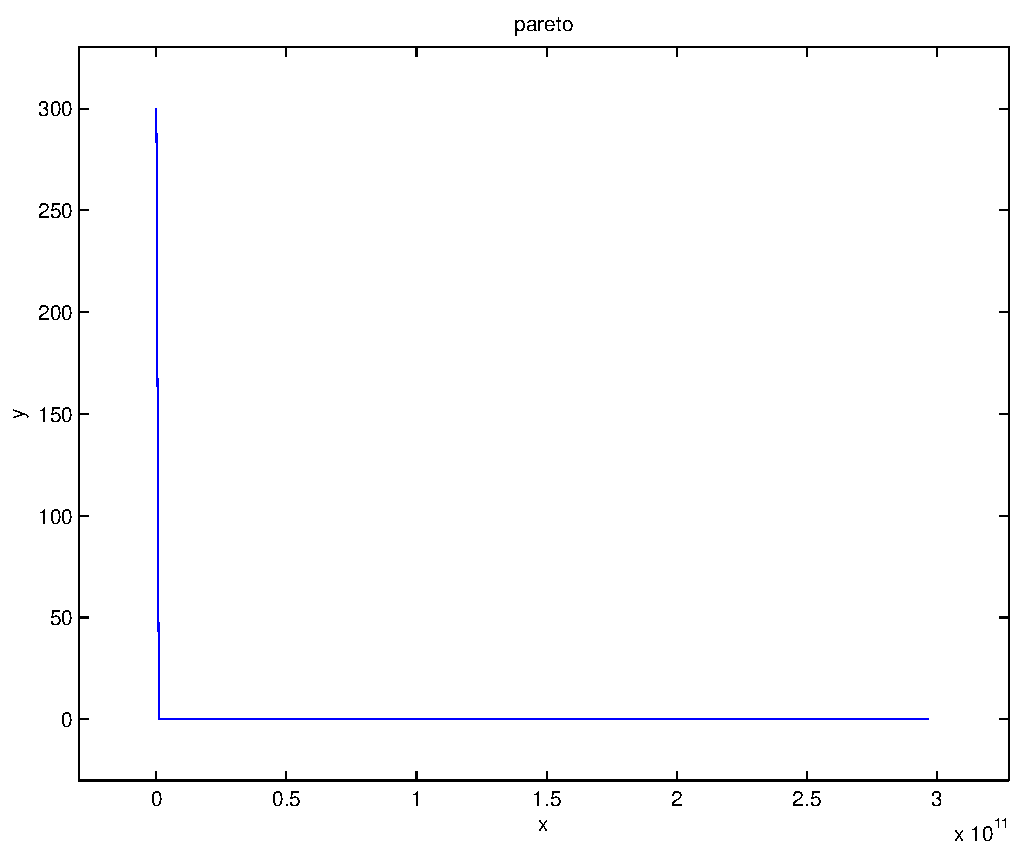
\includegraphics[width=5cm,height=5cm]{pareto.pdf}

poisson \begin{tabular}{|c|c|c|c|}  mean & variance & skewness & kurtosis \\  \hline
$\mu_1 = +1.10545$ & $\mu_2 = +0.13057$ & $\mu_3 = +3.94167$ & $\mu_4 =+21.36551$ \\
\end{tabular}

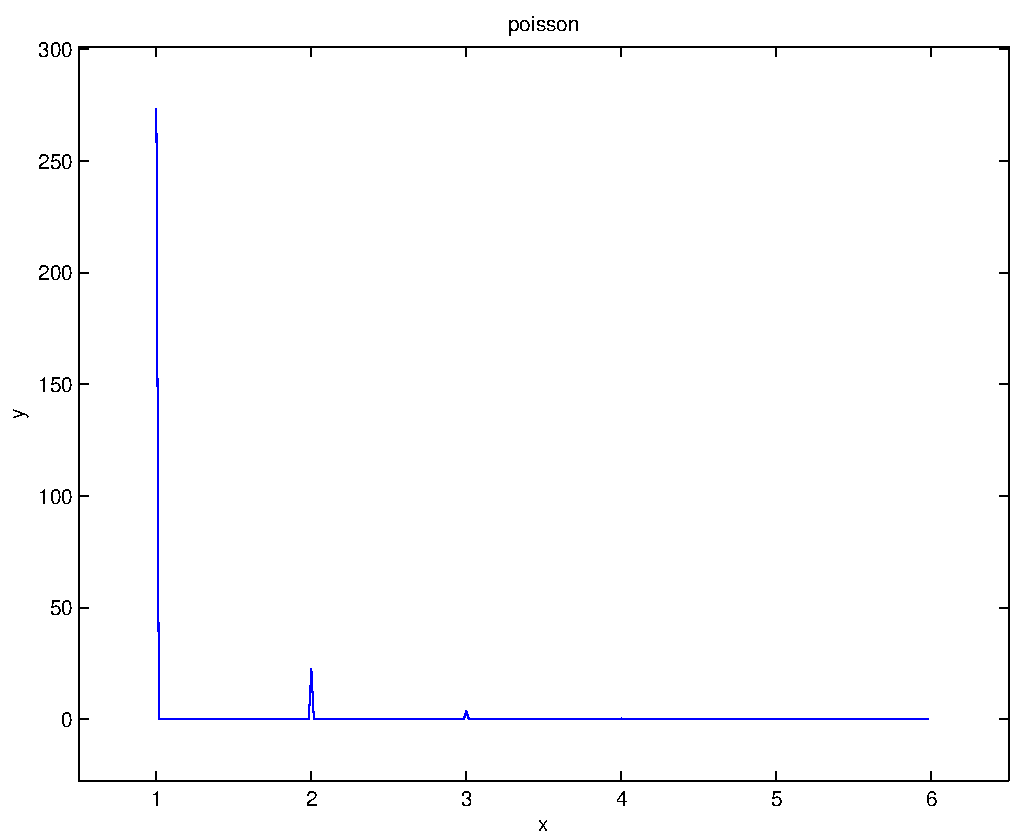
\includegraphics[width=5cm,height=5cm]{poisson.pdf}

\newpage
beta \begin{tabular}{|c|c|c|c|}  mean & variance & skewness & kurtosis \\  \hline
$\mu_1 = +0.33501$ & $\mu_2 = +0.12730$ & $\mu_3 = +0.67247$ & $\mu_4 =+1.89726$ \\
\end{tabular}

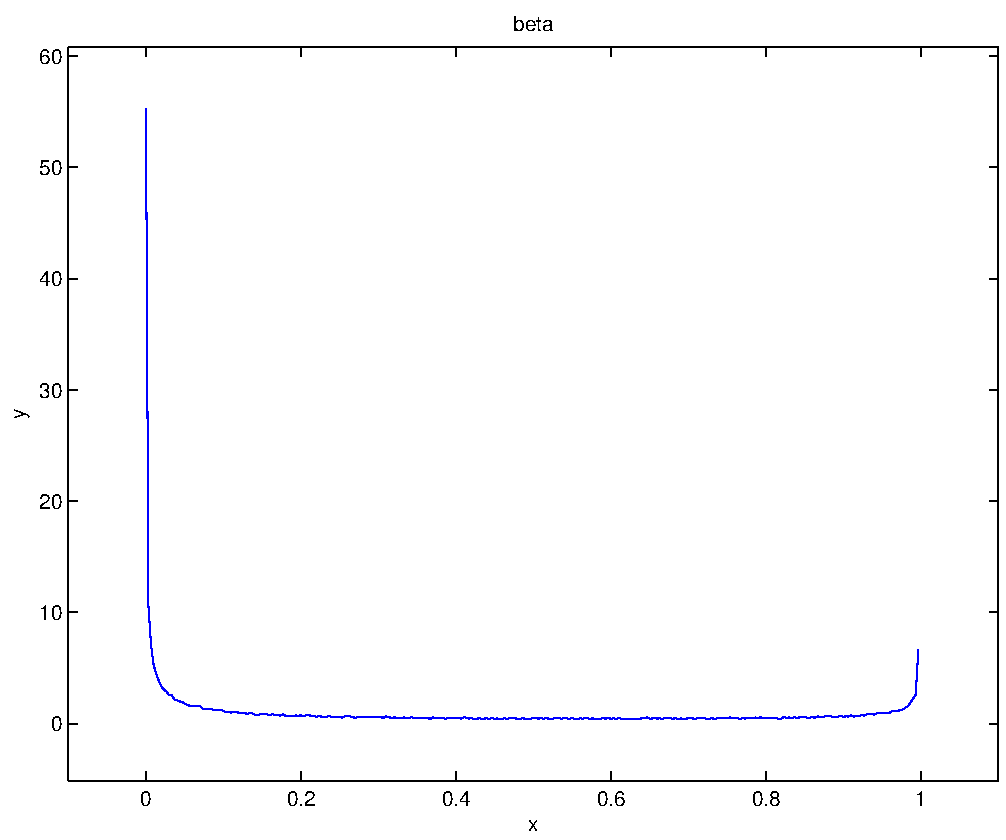
\includegraphics[width=5cm,height=5cm]{beta.pdf}

QueryPerformanceCounter  =  +24.11109
\subsubsection{Multiclass Support Vector Machine }
\begin{itemize}
\item Number or training points = 1024
\item Feature dimension = 3
\item Number or classes = 3
\end{itemize}
{The mean vectors of the 3 classes}

$\mu_1 = \left(
\begin{array}{
ccc}
+1.90000 & +0.10000 & +0.10000 \\
\end{array}
\right)$ \newline 

$\mu_2 = \left(
\begin{array}{
ccc}
+0.10000 & +1.90000 & +0.10000 \\
\end{array}
\right)$ \newline 

$\mu_3 = \left(
\begin{array}{
ccc}
+0.00000 & +0.00000 & +1.90000 \\
\end{array}
\right)$ \newline 

A random SPD covairance matrix is generated for each of the classes.\newline

$\rho_1 = \left(
\begin{array}{
ccc}
+1.651 & -0.339 & -0.142 \\
-0.339 & +1.604 & +0.426 \\
-0.142 & +0.426 & +1.633 \\
\end{array}
\right)$ \newline 

$\rho_2 = \left(
\begin{array}{
ccc}
+4.202 & +0.126 & +0.177 \\
+0.126 & +3.034 & +0.420 \\
+0.177 & +0.420 & +2.012 \\
\end{array}
\right)$ \newline 

$\rho_3 = \left(
\begin{array}{
ccc}
+3.720 & +0.408 & -0.478 \\
+0.408 & +2.946 & -0.254 \\
-0.478 & -0.254 & +3.195 \\
\end{array}
\right)$ \newline 

Verify $L_1$ condition number of covariance. The diagonal entries of the matrix have the form $(0.5 + U(0,1) )*dim(Dom(Cov))$
The lower-diagonal entries take the form $U(0,1) - 0.5$. 
The $L_1$ condition numbers are :
\begin{itemize}
\item +1.856
\item +2.716
\item +1.757
\end{itemize}
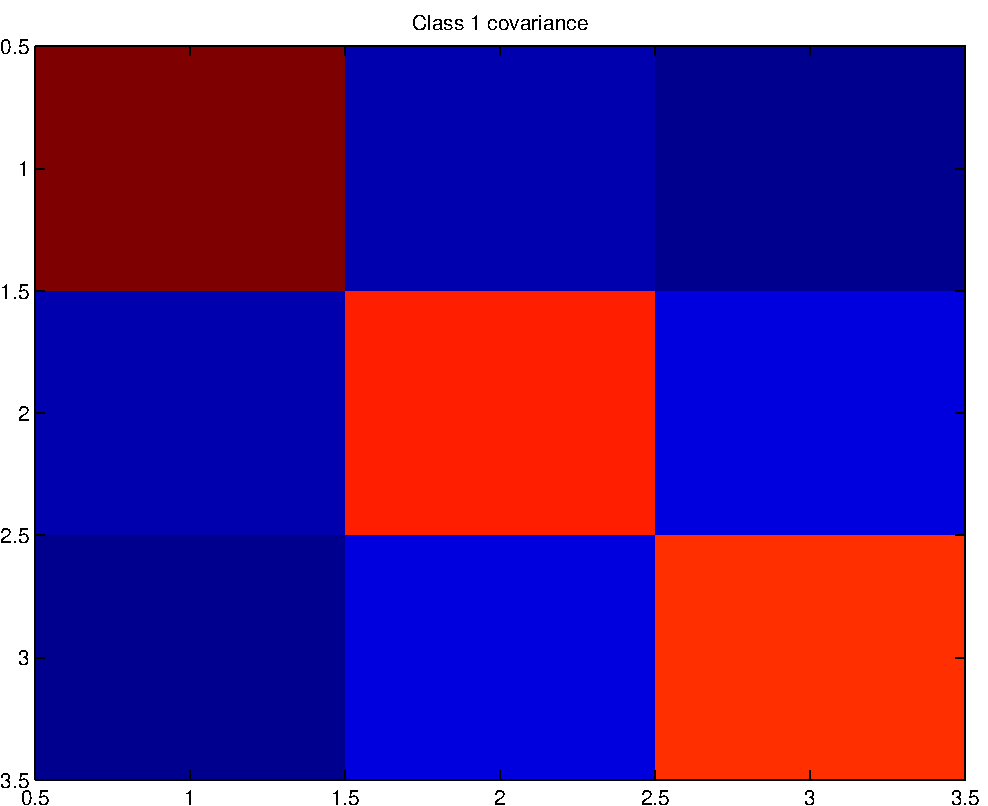
\includegraphics[width=10.0cm,height=10.0cm]{rv1_corr.pdf}

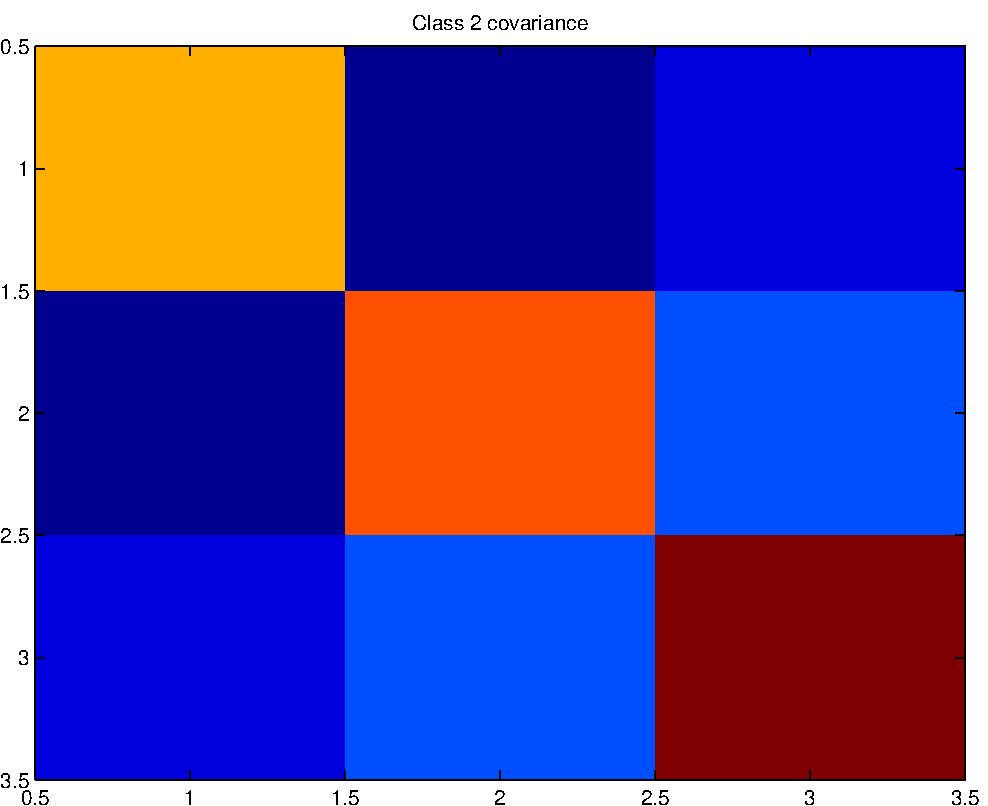
\includegraphics[width=10.0cm,height=10.0cm]{rv2_corr.pdf}

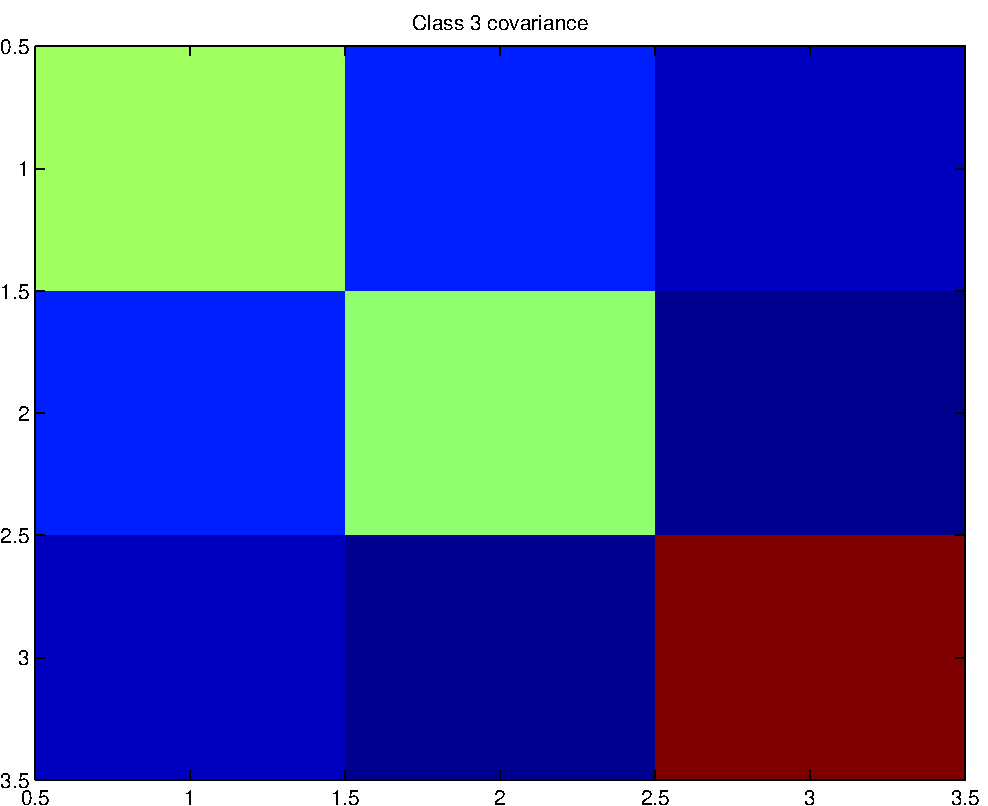
\includegraphics[width=10.0cm,height=10.0cm]{rv3_corr.pdf}

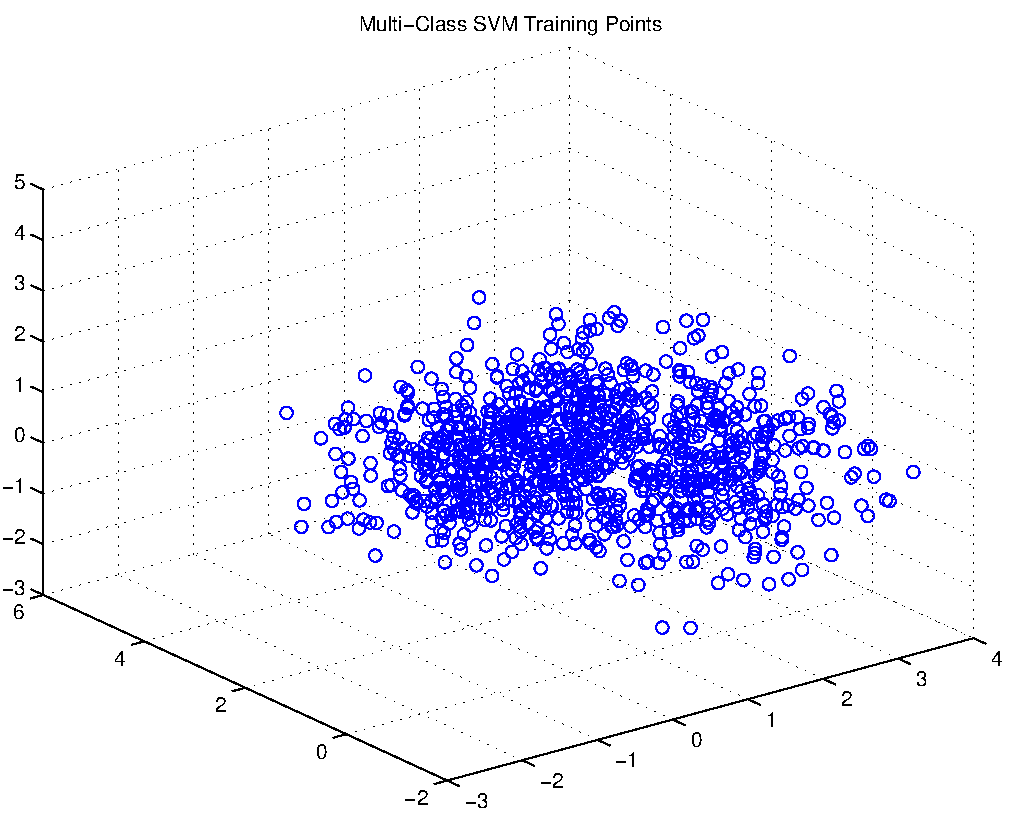
\includegraphics[width=10.0cm,height=10.0cm]{trainingPoints.pdf}

These are the SVM parameters - the RBF kernel is used\begin{itemize}
\item allOutlierFraction=0.05
\item mixingCoeff=0.3
\item smoThresh=1.0/10000.0
\item sigma=1
\end{itemize}
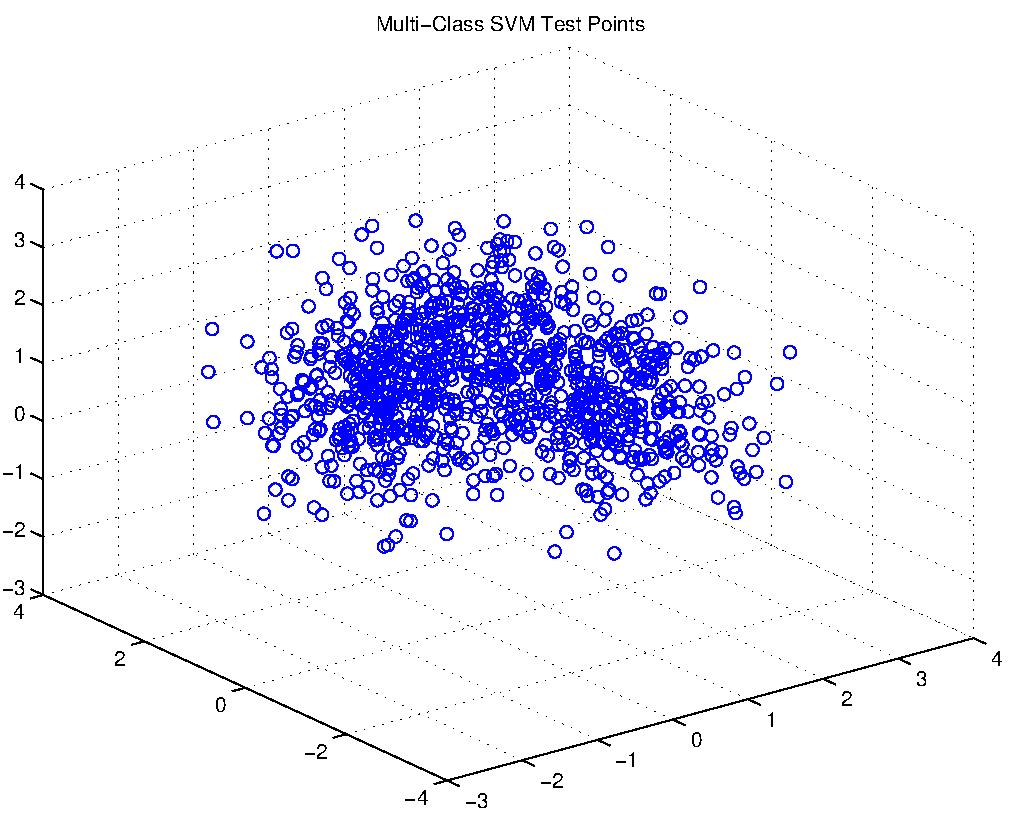
\includegraphics[width=10.0cm,height=10.0cm]{testPoints.pdf}

The marginal sample moments (mean var skew kurtosis) for training points.\newline
\begin{tabular}{ c |  c  c  c  c}
Feature & $\mu_1$ & $\mu_2$ & $\mu_3$ & $\mu_4$ \\
0 & +0.666 & +1.410 & -0.091& +2.208 \\
\hline
1 & +0.700 & +1.210 & +0.476& +2.491 \\
\hline
2 & +0.708 & +1.177 & +0.607& +2.620 \\
\hline
\end{tabular}
\newline
The marginal sample moments (mean var skew kurtosis) for test points.\newline
\begin{tabular}{ c | c  c  c  c}
Feature & $\mu_1$ & $\mu_2$ & $\mu_3$ & $\mu_4$ \\
0 & +0.676 & +1.283 & +0.047& +2.169\\
\hline
1 & +0.671 & +1.200 & +0.509& +2.465\\
\hline
2 & +0.717 & +1.134 & +0.568& +2.559\\
\hline
\end{tabular}\newline
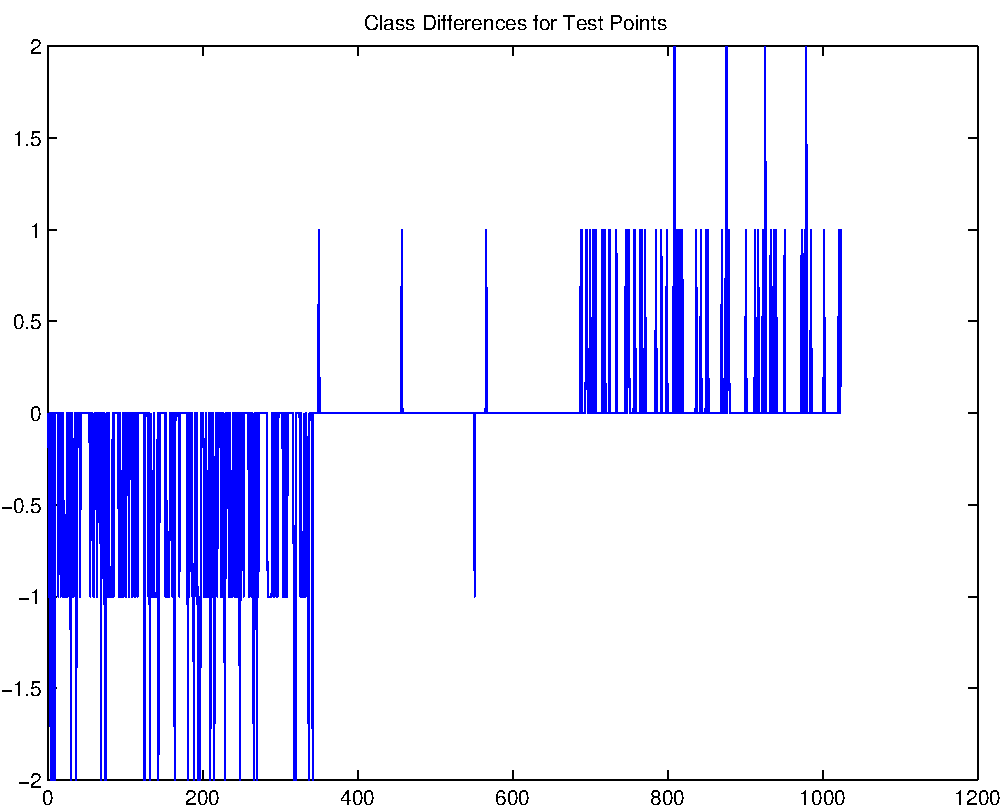
\includegraphics[width=10.0cm,height=10.0cm]{classDiffs.pdf}

The error rate for this run is +0.064\newline
QueryPerformanceCounter  =  +9.336
\subsubsection{Semidefinite Programming SDPA}
QueryPerformanceCounter  =  +0.068
\subsubsection{Linear Regression 3x1}
\subsubsection{3 x 1 Linear Regression}
Sample size = 64

Number of features = 3

$\sigma = \left(
\begin{array}{
ccc}
+3.952 & -0.499 & -0.010 \\
-0.499 & +1.895 & +0.465 \\
-0.010 & +0.465 & +4.477 \\
\end{array}
\right)$ \newline 

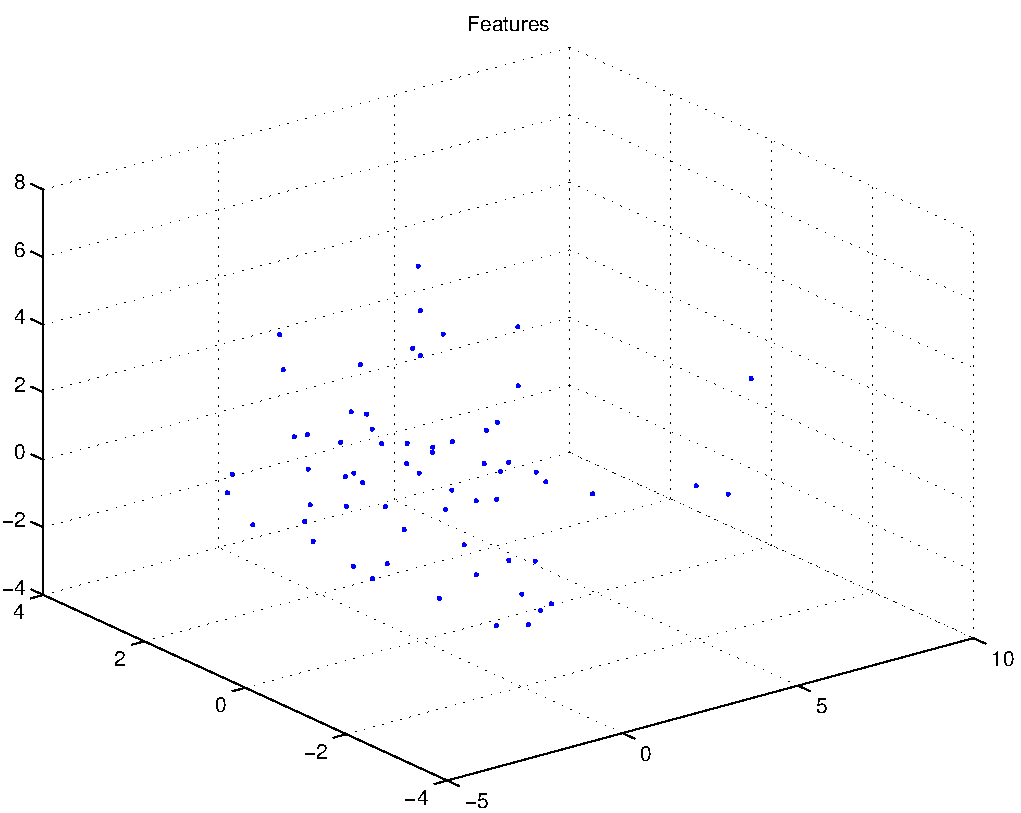
\includegraphics[width=10.0cm,height=10.0cm]{regression_features.pdf}

Beta
+0.817, +0.999, +0.510

Response
-0.857
+1.517
+3.649
+0.487
+0.061
+3.356
-3.453
+1.674
-3.623
+0.850
-1.287
+2.262
-4.347
+3.241
+1.591
+4.218
+0.724
+3.539
-0.392
+3.022
+1.310
+0.448
+0.148
-0.138
-0.852
+2.014
+2.813
-1.806
-2.514
+3.242
-1.518
+4.440
-0.415
+0.663
-6.367
-0.085
-0.088
+2.535
-0.815
+1.259
-0.826
-2.684
+0.991
+2.174
+3.978
+3.591
-2.041
-1.588
-0.583
-2.555
-3.100
-2.562
+0.366
+0.042
+2.006
-0.036
-1.843
+5.234
-0.297
+4.922
+1.822
-1.264
-2.779
-0.047
Estimate for Beta
-6277438562204192200000000000000000000000000000000000000000000000000.000
-6277438562204192200000000000000000000000000000000000000000000000000.000
-6277438562204192200000000000000000000000000000000000000000000000000.000
Error:
+0.000, -0.000, +0.000


QueryPerformanceCounter  =  +1.382
\subsubsection{Matrix Norms}
\subsubsection{Haar Distributed Random Orthogonal Matrix $A \in O(n)$}
 Testing Operator Norm
Number of Dimensions: 12

$A = \left(
\begin{array}{
cccccccccccc}
+0.238 & +0.244 & +0.342 & -0.223 & -0.202 & +0.303 & +0.210 & -0.034 & +0.219 & +0.484 & +0.351 & -0.365 \\
-0.161 & +0.022 & +0.156 & +0.053 & -0.097 & +0.258 & -0.459 & -0.115 & +0.417 & +0.197 & +0.104 & +0.650 \\
-0.010 & +0.490 & -0.118 & +0.270 & +0.549 & -0.103 & -0.169 & -0.478 & -0.173 & +0.220 & +0.140 & -0.072 \\
+0.033 & +0.235 & -0.118 & +0.046 & +0.142 & +0.162 & +0.751 & -0.148 & +0.337 & -0.214 & -0.112 & +0.353 \\
+0.362 & +0.288 & -0.076 & +0.095 & +0.344 & +0.198 & -0.261 & +0.584 & +0.315 & -0.108 & -0.269 & -0.144 \\
+0.157 & +0.109 & +0.134 & +0.637 & -0.356 & -0.487 & +0.124 & +0.132 & +0.101 & +0.312 & -0.174 & +0.069 \\
-0.243 & +0.020 & -0.690 & -0.129 & +0.005 & -0.102 & +0.107 & +0.374 & +0.026 & +0.445 & +0.278 & +0.103 \\
-0.113 & +0.036 & +0.003 & -0.365 & +0.065 & -0.612 & -0.108 & -0.169 & +0.612 & -0.126 & +0.006 & -0.209 \\
-0.564 & +0.491 & -0.109 & +0.162 & -0.420 & +0.213 & -0.095 & +0.015 & +0.053 & -0.280 & -0.068 & -0.293 \\
+0.600 & +0.129 & -0.443 & -0.007 & -0.406 & -0.005 & -0.182 & -0.245 & -0.002 & -0.300 & +0.273 & +0.068 \\
-0.009 & -0.480 & -0.331 & +0.297 & +0.017 & +0.314 & -0.027 & -0.341 & +0.337 & +0.190 & -0.275 & -0.361 \\
+0.104 & +0.245 & -0.119 & -0.439 & -0.192 & -0.003 & -0.056 & -0.178 & -0.184 & +0.324 & -0.706 & +0.116 \\
\end{array}
\right)$ \newline 

$Det(A) :   A \in O(n)$ = (+1.000,+0.000)

$L = \left(
\begin{array}{
cccccccccccc}
+1.000 & +0.000 & +0.000 & +0.000 & +0.000 & +0.000 & +0.000 & +0.000 & +0.000 & +0.000 & +0.000 & +0.000 \\
-0.939 & +1.000 & +0.000 & +0.000 & +0.000 & +0.000 & +0.000 & +0.000 & +0.000 & +0.000 & +0.000 & +0.000 \\
-0.405 & +0.118 & +1.000 & +0.000 & +0.000 & +0.000 & +0.000 & +0.000 & +0.000 & +0.000 & +0.000 & +0.000 \\
+0.261 & +0.123 & -0.390 & +1.000 & +0.000 & +0.000 & +0.000 & +0.000 & +0.000 & +0.000 & +0.000 & +0.000 \\
-0.017 & +0.805 & -0.368 & +0.159 & +1.000 & +0.000 & +0.000 & +0.000 & +0.000 & +0.000 & +0.000 & +0.000 \\
-0.015 & -0.781 & +0.926 & +0.993 & -0.318 & +1.000 & +0.000 & +0.000 & +0.000 & +0.000 & +0.000 & +0.000 \\
+0.055 & +0.372 & -0.126 & -0.053 & +0.373 & +0.115 & +1.000 & +0.000 & +0.000 & +0.000 & +0.000 & +0.000 \\
+0.604 & +0.343 & -0.460 & -0.041 & +0.694 & +0.191 & +0.062 & +1.000 & +0.000 & +0.000 & +0.000 & +0.000 \\
-0.188 & +0.097 & +0.035 & -0.670 & -0.041 & -0.939 & -0.483 & -0.747 & +1.000 & +0.000 & +0.000 & +0.000 \\
+0.396 & +0.316 & -0.846 & -0.706 & +0.027 & -0.240 & +0.495 & +0.167 & +0.063 & +1.000 & +0.000 & +0.000 \\
+0.173 & +0.364 & -0.184 & -0.929 & -0.005 & -0.578 & -0.001 & -0.286 & +0.090 & +0.565 & +1.000 & +0.000 \\
-0.268 & +0.093 & -0.107 & +0.037 & -0.111 & +0.203 & -0.406 & +0.127 & +0.340 & +0.460 & -0.178 & +1.000 \\
\end{array}
\right)$ \newline 

$U = \left(
\begin{array}{
cccccccccccc}
+0.600 & +0.129 & -0.443 & -0.007 & -0.406 & -0.005 & -0.182 & -0.245 & -0.002 & -0.300 & +0.273 & +0.068 \\
+0.000 & +0.612 & -0.524 & +0.156 & -0.801 & +0.208 & -0.266 & -0.215 & +0.051 & -0.562 & +0.188 & -0.229 \\
+0.000 & +0.000 & -0.807 & -0.150 & -0.065 & -0.128 & +0.065 & +0.300 & +0.019 & +0.390 & +0.367 & +0.157 \\
+0.000 & +0.000 & +0.000 & +0.562 & -0.177 & -0.561 & +0.230 & +0.339 & +0.103 & +0.611 & -0.126 & +0.141 \\
+0.000 & +0.000 & +0.000 & +0.000 & +1.191 & -0.228 & +0.030 & -0.253 & -0.223 & +0.714 & +0.148 & +0.148 \\
+0.000 & +0.000 & +0.000 & +0.000 & +0.000 & +1.079 & -0.516 & -1.207 & +0.187 & -0.994 & -0.291 & -0.777 \\
+0.000 & +0.000 & +0.000 & +0.000 & +0.000 & +0.000 & +0.928 & +0.235 & +0.387 & -0.059 & -0.180 & +0.495 \\
+0.000 & +0.000 & +0.000 & +0.000 & +0.000 & +0.000 & +0.000 & +1.349 & +0.407 & +0.168 & -0.371 & -0.014 \\
+0.000 & +0.000 & +0.000 & +0.000 & +0.000 & +0.000 & +0.000 & +0.000 & +1.332 & -0.539 & -0.689 & -0.580 \\
+0.000 & +0.000 & +0.000 & +0.000 & +0.000 & +0.000 & +0.000 & +0.000 & +0.000 & +1.319 & +0.525 & -0.484 \\
+0.000 & +0.000 & +0.000 & +0.000 & +0.000 & +0.000 & +0.000 & +0.000 & +0.000 & +0.000 & -1.380 & +0.221 \\
+0.000 & +0.000 & +0.000 & +0.000 & +0.000 & +0.000 & +0.000 & +0.000 & +0.000 & +0.000 & +0.000 & +1.538 \\
\end{array}
\right)$ \newline 

$L * U  = \left(
\begin{array}{
cccccccccccc}
+0.600 & +0.129 & -0.443 & -0.007 & -0.406 & -0.005 & -0.182 & -0.245 & -0.002 & -0.300 & +0.273 & +0.068 \\
-0.564 & +0.491 & -0.109 & +0.162 & -0.420 & +0.213 & -0.095 & +0.015 & +0.053 & -0.280 & -0.068 & -0.293 \\
-0.243 & +0.020 & -0.690 & -0.129 & +0.005 & -0.102 & +0.107 & +0.374 & +0.026 & +0.445 & +0.278 & +0.103 \\
+0.157 & +0.109 & +0.134 & +0.637 & -0.356 & -0.487 & +0.124 & +0.132 & +0.101 & +0.312 & -0.174 & +0.069 \\
-0.010 & +0.490 & -0.118 & +0.270 & +0.549 & -0.103 & -0.169 & -0.478 & -0.173 & +0.220 & +0.140 & -0.072 \\
-0.009 & -0.480 & -0.331 & +0.297 & +0.017 & +0.314 & -0.027 & -0.341 & +0.337 & +0.190 & -0.275 & -0.361 \\
+0.033 & +0.235 & -0.118 & +0.046 & +0.142 & +0.162 & +0.751 & -0.148 & +0.337 & -0.214 & -0.112 & +0.353 \\
+0.362 & +0.288 & -0.076 & +0.095 & +0.344 & +0.198 & -0.261 & +0.584 & +0.315 & -0.108 & -0.269 & -0.144 \\
-0.113 & +0.036 & +0.003 & -0.365 & +0.065 & -0.612 & -0.108 & -0.169 & +0.612 & -0.126 & +0.006 & -0.209 \\
+0.238 & +0.244 & +0.342 & -0.223 & -0.202 & +0.303 & +0.210 & -0.034 & +0.219 & +0.484 & +0.351 & -0.365 \\
+0.104 & +0.245 & -0.119 & -0.439 & -0.192 & -0.003 & -0.056 & -0.178 & -0.184 & +0.324 & -0.706 & +0.116 \\
-0.161 & +0.022 & +0.156 & +0.053 & -0.097 & +0.258 & -0.459 & -0.115 & +0.417 & +0.197 & +0.104 & +0.650 \\
\end{array}
\right)$ \newline 

$Det(L) :    = (+1.000,+0.000)     Det(U) :    = (+1.000,+0.000)     Det(LU) :    = (+1.000,+0.000)$

$||A||_{L_1}$  = +3.200

$||A||_{L_{\infty}}$ = +3.215

$||A^{-1}||_{L_1}$  = +3.215

$||A^{-1}||_{L_{\infty}}$ = +3.200

$||A||_{L_{\infty}} * ||A^{-1}||_{L_{\infty}} = +10.290$

$||A||_{L_1} * ||A^{-1}||_{L_1} = +10.290$

Frobenious Norm  $||A||_{\textit{F}}$ via $\sum\limits_{i,j =0}^{n} \|A_{i,j}|$   of  $A \in O(n)$  +3.464

$L_1$ condition number of Haar Distributed Random Orthogonal Matrix $A \in O(n)$ +9.534

$A = \left(
\begin{array}{
cccccccccccc}
+0.238 & +0.244 & +0.342 & -0.223 & -0.202 & +0.303 & +0.210 & -0.034 & +0.219 & +0.484 & +0.351 & -0.365 \\
-0.161 & +0.022 & +0.156 & +0.053 & -0.097 & +0.258 & -0.459 & -0.115 & +0.417 & +0.197 & +0.104 & +0.650 \\
-0.010 & +0.490 & -0.118 & +0.270 & +0.549 & -0.103 & -0.169 & -0.478 & -0.173 & +0.220 & +0.140 & -0.072 \\
+0.033 & +0.235 & -0.118 & +0.046 & +0.142 & +0.162 & +0.751 & -0.148 & +0.337 & -0.214 & -0.112 & +0.353 \\
+0.362 & +0.288 & -0.076 & +0.095 & +0.344 & +0.198 & -0.261 & +0.584 & +0.315 & -0.108 & -0.269 & -0.144 \\
+0.157 & +0.109 & +0.134 & +0.637 & -0.356 & -0.487 & +0.124 & +0.132 & +0.101 & +0.312 & -0.174 & +0.069 \\
-0.243 & +0.020 & -0.690 & -0.129 & +0.005 & -0.102 & +0.107 & +0.374 & +0.026 & +0.445 & +0.278 & +0.103 \\
-0.113 & +0.036 & +0.003 & -0.365 & +0.065 & -0.612 & -0.108 & -0.169 & +0.612 & -0.126 & +0.006 & -0.209 \\
-0.564 & +0.491 & -0.109 & +0.162 & -0.420 & +0.213 & -0.095 & +0.015 & +0.053 & -0.280 & -0.068 & -0.293 \\
+0.600 & +0.129 & -0.443 & -0.007 & -0.406 & -0.005 & -0.182 & -0.245 & -0.002 & -0.300 & +0.273 & +0.068 \\
-0.009 & -0.480 & -0.331 & +0.297 & +0.017 & +0.314 & -0.027 & -0.341 & +0.337 & +0.190 & -0.275 & -0.361 \\
+0.104 & +0.245 & -0.119 & -0.439 & -0.192 & -0.003 & -0.056 & -0.178 & -0.184 & +0.324 & -0.706 & +0.116 \\
\end{array}
\right)$ \newline 

$L_{\infty}$ condition number of Haar Distributed Random Orthogonal Matrix $A \in O(n)$ +10.290

Eigenvalues of $A \in O(n)$

(+0.283,+0.959), (+0.283,-0.959), (-0.472,+0.881), (-0.472,-0.881), (-0.823,+0.568), (-0.823,-0.568), (-0.920,+0.392), (-0.920,-0.392), (+0.971,+0.237), (+0.971,-0.237), (+0.751,+0.661), (+0.751,-0.661)

 $|\lambda | : \lambda \in \sigma(A) , A \in O(n)$

+1.000, +1.000, +1.000, +1.000, +1.000, +1.000, +1.000, +1.000, +1.000, +1.000, +1.000, +1.000


Calculating $A^{\dag} A,$  we expect $A^{\dag} A \approx I$

$A^{\dag} A = \left(
\begin{array}{
cccccccccccc}
+1.000 & -0.000 & -0.000 & +0.000 & -0.000 & +0.000 & +0.000 & -0.000 & +0.000 & -0.000 & +0.000 & -0.000 \\
-0.000 & +1.000 & +0.000 & +0.000 & +0.000 & -0.000 & -0.000 & -0.000 & +0.000 & -0.000 & -0.000 & +0.000 \\
-0.000 & +0.000 & +1.000 & +0.000 & -0.000 & +0.000 & -0.000 & -0.000 & +0.000 & +0.000 & +0.000 & -0.000 \\
+0.000 & +0.000 & +0.000 & +1.000 & +0.000 & -0.000 & +0.000 & +0.000 & -0.000 & +0.000 & -0.000 & +0.000 \\
-0.000 & +0.000 & -0.000 & +0.000 & +1.000 & +0.000 & -0.000 & -0.000 & +0.000 & +0.000 & -0.000 & -0.000 \\
+0.000 & -0.000 & +0.000 & -0.000 & +0.000 & +1.000 & +0.000 & -0.000 & -0.000 & +0.000 & -0.000 & +0.000 \\
+0.000 & -0.000 & -0.000 & +0.000 & -0.000 & +0.000 & +1.000 & +0.000 & -0.000 & -0.000 & +0.000 & -0.000 \\
-0.000 & -0.000 & -0.000 & +0.000 & -0.000 & -0.000 & +0.000 & +1.000 & -0.000 & -0.000 & +0.000 & -0.000 \\
+0.000 & +0.000 & +0.000 & -0.000 & +0.000 & -0.000 & -0.000 & -0.000 & +1.000 & +0.000 & -0.000 & +0.000 \\
-0.000 & -0.000 & +0.000 & +0.000 & +0.000 & +0.000 & -0.000 & -0.000 & +0.000 & +1.000 & +0.000 & -0.000 \\
+0.000 & -0.000 & +0.000 & -0.000 & -0.000 & -0.000 & +0.000 & +0.000 & -0.000 & +0.000 & +1.000 & +0.000 \\
-0.000 & +0.000 & -0.000 & +0.000 & -0.000 & +0.000 & -0.000 & -0.000 & +0.000 & -0.000 & +0.000 & +1.000 \\
\end{array}
\right)$ \newline 

Calculating $A^{-1} ,  A \in O(n)$.

$A^{-1} = \left(
\begin{array}{
cccccccccccc}
+0.238 & -0.161 & -0.010 & +0.033 & +0.362 & +0.157 & -0.243 & -0.113 & -0.564 & +0.600 & -0.009 & +0.104 \\
+0.244 & +0.022 & +0.490 & +0.235 & +0.288 & +0.109 & +0.020 & +0.036 & +0.491 & +0.129 & -0.480 & +0.245 \\
+0.342 & +0.156 & -0.118 & -0.118 & -0.076 & +0.134 & -0.690 & +0.003 & -0.109 & -0.443 & -0.331 & -0.119 \\
-0.223 & +0.053 & +0.270 & +0.046 & +0.095 & +0.637 & -0.129 & -0.365 & +0.162 & -0.007 & +0.297 & -0.439 \\
-0.202 & -0.097 & +0.549 & +0.142 & +0.344 & -0.356 & +0.005 & +0.065 & -0.420 & -0.406 & +0.017 & -0.192 \\
+0.303 & +0.258 & -0.103 & +0.162 & +0.198 & -0.487 & -0.102 & -0.612 & +0.213 & -0.005 & +0.314 & -0.003 \\
+0.210 & -0.459 & -0.169 & +0.751 & -0.261 & +0.124 & +0.107 & -0.108 & -0.095 & -0.182 & -0.027 & -0.056 \\
-0.034 & -0.115 & -0.478 & -0.148 & +0.584 & +0.132 & +0.374 & -0.169 & +0.015 & -0.245 & -0.341 & -0.178 \\
+0.219 & +0.417 & -0.173 & +0.337 & +0.315 & +0.101 & +0.026 & +0.612 & +0.053 & -0.002 & +0.337 & -0.184 \\
+0.484 & +0.197 & +0.220 & -0.214 & -0.108 & +0.312 & +0.445 & -0.126 & -0.280 & -0.300 & +0.190 & +0.324 \\
+0.351 & +0.104 & +0.140 & -0.112 & -0.269 & -0.174 & +0.278 & +0.006 & -0.068 & +0.273 & -0.275 & -0.706 \\
-0.365 & +0.650 & -0.072 & +0.353 & -0.144 & +0.069 & +0.103 & -0.209 & -0.293 & +0.068 & -0.361 & +0.116 \\
\end{array}
\right)$ \newline 

Calculating $A^{-1} *A  ,  A \in O(n)$.   We expect $A^{-1} *A  \approx I$. 

$A^{-1} *A = \left(
\begin{array}{
cccccccccccc}
+1.000 & +0.000 & -0.000 & -0.000 & -0.000 & +0.000 & -0.000 & -0.000 & +0.000 & -0.000 & +0.000 & -0.000 \\
+0.000 & +1.000 & +0.000 & -0.000 & +0.000 & +0.000 & +0.000 & -0.000 & +0.000 & -0.000 & -0.000 & +0.000 \\
+0.000 & +0.000 & +1.000 & -0.000 & -0.000 & +0.000 & -0.000 & -0.000 & -0.000 & +0.000 & +0.000 & +0.000 \\
+0.000 & +0.000 & +0.000 & +1.000 & +0.000 & +0.000 & -0.000 & -0.000 & +0.000 & -0.000 & -0.000 & -0.000 \\
-0.000 & -0.000 & +0.000 & +0.000 & +1.000 & +0.000 & -0.000 & +0.000 & +0.000 & -0.000 & -0.000 & -0.000 \\
-0.000 & -0.000 & -0.000 & +0.000 & -0.000 & +1.000 & -0.000 & +0.000 & +0.000 & -0.000 & -0.000 & +0.000 \\
-0.000 & -0.000 & +0.000 & -0.000 & -0.000 & -0.000 & +1.000 & -0.000 & -0.000 & -0.000 & +0.000 & +0.000 \\
+0.000 & +0.000 & -0.000 & -0.000 & -0.000 & +0.000 & -0.000 & +1.000 & +0.000 & +0.000 & -0.000 & +0.000 \\
+0.000 & +0.000 & -0.000 & -0.000 & -0.000 & -0.000 & -0.000 & +0.000 & +1.000 & -0.000 & -0.000 & -0.000 \\
+0.000 & +0.000 & -0.000 & +0.000 & +0.000 & -0.000 & +0.000 & -0.000 & +0.000 & +1.000 & +0.000 & -0.000 \\
-0.000 & -0.000 & -0.000 & +0.000 & +0.000 & +0.000 & +0.000 & -0.000 & -0.000 & -0.000 & +1.000 & +0.000 \\
-0.000 & -0.000 & -0.000 & -0.000 & -0.000 & +0.000 & -0.000 & +0.000 & -0.000 & +0.000 & +0.000 & +1.000 \\
\end{array}
\right)$ \newline 

Calculating SVD of  $A \in O(n)$

$U = \left(
\begin{array}{
cccccccccccc}
-0.091 & +0.066 & -0.281 & -0.694 & +0.052 & -0.168 & +0.012 & -0.345 & +0.178 & +0.025 & -0.425 & -0.252 \\
+0.214 & -0.274 & -0.325 & +0.179 & +0.041 & -0.279 & +0.657 & -0.146 & -0.348 & +0.160 & +0.088 & -0.233 \\
+0.030 & -0.311 & +0.422 & -0.335 & -0.443 & -0.009 & +0.105 & -0.315 & -0.342 & -0.100 & +0.022 & +0.421 \\
-0.238 & -0.244 & -0.342 & +0.223 & +0.202 & -0.303 & -0.210 & +0.034 & -0.219 & -0.484 & -0.351 & +0.365 \\
+0.820 & -0.259 & -0.063 & -0.011 & +0.100 & +0.298 & -0.069 & -0.006 & +0.207 & -0.246 & -0.216 & +0.051 \\
+0.028 & +0.502 & +0.206 & +0.250 & -0.249 & +0.172 & +0.197 & -0.059 & -0.293 & -0.320 & -0.492 & -0.280 \\
+0.157 & +0.083 & +0.412 & +0.064 & +0.032 & -0.696 & +0.095 & -0.042 & +0.394 & -0.336 & +0.132 & -0.115 \\
-0.308 & -0.254 & +0.132 & +0.057 & +0.330 & +0.396 & +0.104 & -0.433 & +0.084 & -0.432 & +0.271 & -0.297 \\
-0.185 & -0.473 & +0.332 & +0.325 & -0.014 & -0.007 & -0.026 & -0.063 & +0.246 & +0.411 & -0.522 & -0.140 \\
+0.161 & +0.089 & +0.391 & -0.163 & +0.679 & -0.104 & -0.174 & +0.017 & -0.491 & +0.187 & -0.072 & -0.049 \\
+0.089 & -0.264 & -0.064 & +0.001 & -0.338 & -0.151 & -0.566 & +0.056 & -0.298 & -0.078 & +0.154 & -0.582 \\
-0.164 & -0.270 & +0.140 & -0.350 & +0.019 & +0.097 & +0.312 & +0.747 & -0.016 & -0.239 & -0.084 & -0.168 \\
\end{array}
\right)$ \newline 

$S = \left(
\begin{array}{
cccccccccccc}
+1.000 & +0.000 & +0.000 & +0.000 & +0.000 & +0.000 & +0.000 & +0.000 & +0.000 & +0.000 & +0.000 & +0.000 \\
+0.000 & +1.000 & +0.000 & +0.000 & +0.000 & +0.000 & +0.000 & +0.000 & +0.000 & +0.000 & +0.000 & +0.000 \\
+0.000 & +0.000 & +1.000 & +0.000 & +0.000 & +0.000 & +0.000 & +0.000 & +0.000 & +0.000 & +0.000 & +0.000 \\
+0.000 & +0.000 & +0.000 & +1.000 & +0.000 & +0.000 & +0.000 & +0.000 & +0.000 & +0.000 & +0.000 & +0.000 \\
+0.000 & +0.000 & +0.000 & +0.000 & +1.000 & +0.000 & +0.000 & +0.000 & +0.000 & +0.000 & +0.000 & +0.000 \\
+0.000 & +0.000 & +0.000 & +0.000 & +0.000 & +1.000 & +0.000 & +0.000 & +0.000 & +0.000 & +0.000 & +0.000 \\
+0.000 & +0.000 & +0.000 & +0.000 & +0.000 & +0.000 & +1.000 & +0.000 & +0.000 & +0.000 & +0.000 & +0.000 \\
+0.000 & +0.000 & +0.000 & +0.000 & +0.000 & +0.000 & +0.000 & +1.000 & +0.000 & +0.000 & +0.000 & +0.000 \\
+0.000 & +0.000 & +0.000 & +0.000 & +0.000 & +0.000 & +0.000 & +0.000 & +1.000 & +0.000 & +0.000 & +0.000 \\
+0.000 & +0.000 & +0.000 & +0.000 & +0.000 & +0.000 & +0.000 & +0.000 & +0.000 & +1.000 & +0.000 & +0.000 \\
+0.000 & +0.000 & +0.000 & +0.000 & +0.000 & +0.000 & +0.000 & +0.000 & +0.000 & +0.000 & +1.000 & +0.000 \\
+0.000 & +0.000 & +0.000 & +0.000 & +0.000 & +0.000 & +0.000 & +0.000 & +0.000 & +0.000 & +0.000 & +1.000 \\
\end{array}
\right)$ \newline 

$V = \left(
\begin{array}{
cccccccccccc}
+0.000 & -0.000 & -0.000 & -1.000 & +0.000 & -0.000 & +0.000 & -0.000 & -0.000 & +0.000 & +0.000 & -0.000 \\
-0.208 & -0.699 & +0.179 & -0.000 & +0.000 & -0.381 & -0.140 & -0.075 & +0.145 & -0.194 & -0.285 & -0.354 \\
+0.022 & +0.085 & -0.393 & -0.000 & -0.216 & +0.061 & -0.014 & +0.158 & -0.169 & +0.477 & -0.126 & -0.701 \\
+0.067 & +0.222 & -0.024 & +0.000 & +0.149 & +0.182 & +0.097 & +0.156 & -0.150 & -0.295 & -0.864 & +0.037 \\
-0.074 & -0.374 & -0.672 & +0.000 & +0.477 & +0.139 & +0.021 & -0.235 & -0.040 & +0.159 & -0.047 & +0.267 \\
-0.385 & +0.241 & -0.094 & +0.000 & -0.119 & +0.205 & +0.367 & -0.571 & +0.402 & -0.210 & -0.014 & -0.249 \\
+0.067 & +0.251 & -0.373 & +0.000 & -0.358 & -0.506 & -0.378 & -0.363 & -0.231 & -0.238 & -0.068 & +0.139 \\
+0.584 & -0.157 & -0.156 & +0.000 & -0.119 & -0.292 & +0.696 & +0.016 & +0.028 & -0.145 & +0.052 & -0.026 \\
+0.043 & -0.333 & -0.215 & +0.000 & -0.477 & +0.560 & -0.113 & +0.167 & -0.131 & -0.466 & +0.159 & +0.004 \\
+0.004 & +0.098 & +0.097 & +0.000 & +0.477 & +0.011 & +0.034 & -0.142 & -0.572 & -0.390 & +0.301 & -0.403 \\
+0.195 & +0.208 & -0.289 & +0.000 & +0.298 & -0.094 & -0.290 & +0.352 & +0.589 & -0.337 & +0.143 & -0.218 \\
+0.642 & -0.076 & +0.223 & +0.000 & +0.060 & +0.304 & -0.330 & -0.509 & +0.138 & +0.137 & -0.107 & -0.135 \\
\end{array}
\right)$ \newline 

$U S V = \left(
\begin{array}{
cccccccccccc}
-0.444 & -0.353 & +0.200 & +0.091 & -0.176 & -0.037 & -0.191 & -0.079 & -0.244 & +0.165 & +0.599 & +0.332 \\
-0.021 & +0.476 & -0.137 & -0.214 & +0.186 & -0.497 & -0.295 & -0.026 & -0.308 & -0.187 & -0.057 & +0.454 \\
+0.171 & +0.495 & +0.247 & -0.030 & -0.204 & -0.008 & -0.377 & -0.145 & +0.088 & +0.561 & +0.196 & -0.313 \\
+0.320 & -0.090 & +0.234 & +0.238 & +0.101 & +0.192 & +0.046 & -0.076 & +0.057 & +0.419 & -0.339 & +0.655 \\
-0.080 & +0.050 & -0.084 & -0.820 & -0.228 & +0.354 & +0.184 & -0.193 & +0.099 & +0.073 & +0.009 & +0.219 \\
-0.442 & -0.099 & +0.202 & -0.028 & -0.386 & -0.422 & +0.150 & -0.112 & -0.075 & +0.202 & -0.575 & -0.120 \\
+0.211 & -0.286 & -0.315 & -0.157 & -0.326 & +0.001 & -0.387 & +0.642 & -0.168 & +0.183 & -0.139 & +0.004 \\
-0.500 & +0.277 & -0.533 & +0.308 & -0.078 & +0.243 & -0.154 & +0.023 & +0.397 & +0.100 & -0.090 & +0.170 \\
-0.086 & +0.297 & -0.087 & +0.185 & -0.098 & +0.436 & +0.240 & +0.025 & -0.766 & +0.051 & -0.085 & -0.089 \\
-0.099 & -0.220 & -0.384 & -0.161 & +0.587 & -0.165 & +0.119 & -0.117 & -0.149 & +0.559 & +0.022 & -0.184 \\
-0.226 & +0.286 & +0.304 & -0.089 & +0.183 & -0.070 & +0.408 & +0.694 & +0.151 & +0.163 & +0.156 & +0.081 \\
+0.328 & +0.077 & -0.382 & +0.164 & -0.427 & -0.361 & +0.514 & -0.086 & +0.043 & +0.128 & +0.308 & +0.127 \\
\end{array}
\right)$ \newline 

\subsubsection{Wishart Matrix $A \in W(n)$}
$L_1$ condition number of Wishart Matrix +56267.800
$L_infty$ condition number of Wishart Matrix +56267.800
\subsubsection{Gaussian Orthogonal Ensemble $A \in GOE(n)$}
$L_1$ condition number of GOE Matrix +470.231
$L_\infty$ condition number of GOE Matrix +470.231
\subsubsection{The Identity Matrix $I \in M(n)$}
$L_1$ condition number of $I$ = +1.000
$L_\infty$ condition number of $I$ = +1.000
QueryPerformanceCounter  =  +1.815
\subsubsection{Principal Components Matlab }
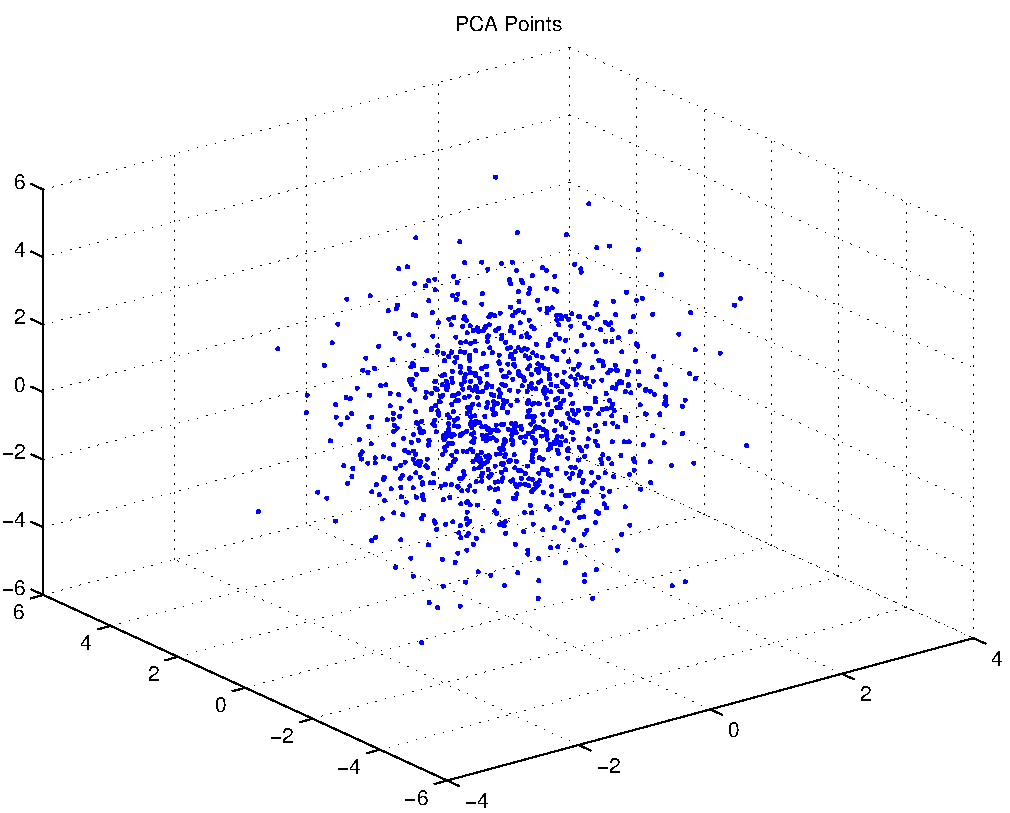
\includegraphics[width=10.0cm,height=10.0cm]{PCAPoints.pdf}

The eigenvectors:
+0.065, +0.220, +0.973
+0.087, +0.970, -0.225
-0.994, +0.099, +0.044

All of the eigenvalues of the covariance matrix:
(+0.958,+0.000), (+2.025,+0.000), (+3.017,+0.000)

QueryPerformanceCounter  =  +1.423
\subsubsection{Multi Variate Random Number Generator }
Sample from $N(\mu,\Sigma)$
mean= -0.002, variance=+1.004, skewness=+0.006, kurtosis=+3.003
mean= -0.001, variance=+1.017, skewness=-0.005, kurtosis=+2.988
mean= -0.002, variance=+1.006, skewness=-0.016, kurtosis=+3.014
Covariance Matrix 
+1.004, +0.009, +0.003
+0.009, +1.017, -0.003
+0.003, -0.003, +1.006

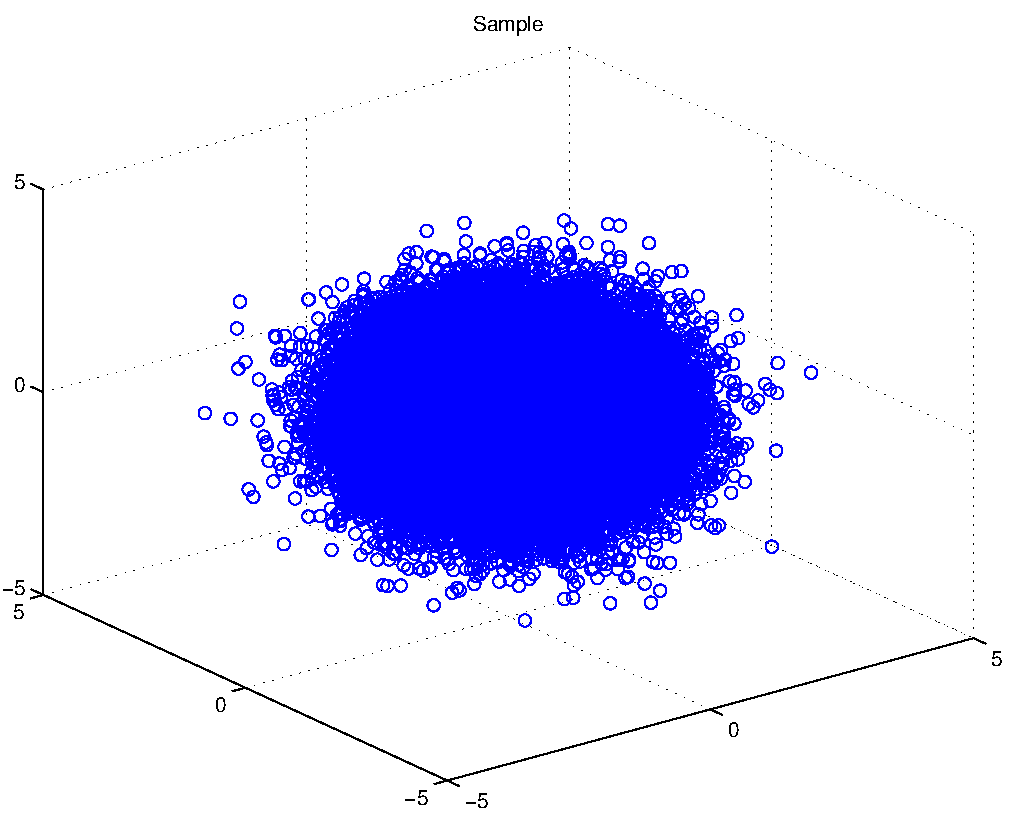
\includegraphics[width=10.0cm,height=10.0cm]{R_3_Normal.pdf}

Generate a sample from a unifom mixture of three Gaussians in $R^3$
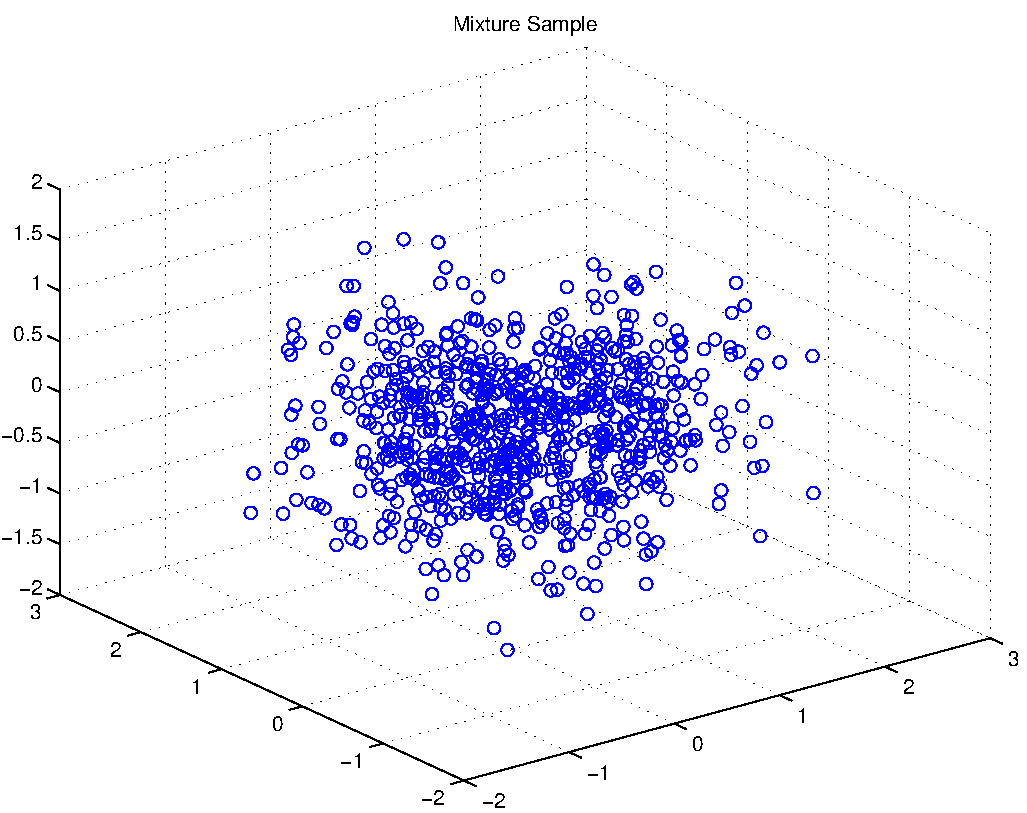
\includegraphics[width=10.0cm,height=10.0cm]{R_3_Normal_Mixture.pdf}

QueryPerformanceCounter  =  +33.721
\subsubsection{Matrix Multiply}
Comparing naive matrix multiply verus Intel MKL dgemm for matrix of size 2048.
This is for type double (hence the d in dgemm).
Naive type double matrix multiply tic toc  =  +3.607
dgemm plus row to column major transpose operation tic toc  =  +2.536
Comparing naive matrix multiply verus Intel MKL sgemm for matrix of size 2048.
This is for type float (hence the s in dgemm).
Naive type float matrix multiply tic toc  =  +3.601
sgemm plus row to column major transpose operation tic toc  =  +2.539
QueryPerformanceCounter  =  +13.613
\subsubsection{Descriptive Statistics}
Mean N(0,1): +0.003
Variance N(0,1): +1.006
Mean N(0,1) [recurrence relation method] :+0.003
Variance [recurrence relation method] :+1.006
Skewness : +0.007
Kurtosis : +2.997
QueryPerformanceCounter  =  +0.053
\subsubsection{Time Series }
+0.093
+0.726
+0.011
+2.178
QueryPerformanceCounter  =  +0.203
\subsubsection{Matrix}
QueryPerformanceCounter  =  +1.342
QueryPerformanceCounter  =  +1.308
\end{document}
